\documentclass[12pt,a4paper,oneside]{report}

% --- Packages ---
\usepackage{amsmath,amssymb}
\usepackage{parskip}
\usepackage{graphicx}
\usepackage{xcolor}
\usepackage[a4paper,margin=1in]{geometry}
\usepackage{longtable,booktabs,array}

\setlength{\parskip}{0.8\baselineskip}

% Encourage figures to share pages with surrounding text instead of sitting alone
\setcounter{topnumber}{2}
\setcounter{bottomnumber}{2}
\setcounter{totalnumber}{4}
\renewcommand{\topfraction}{0.95}
\renewcommand{\bottomfraction}{0.95}
\renewcommand{\textfraction}{0.05}
\renewcommand{\floatpagefraction}{0.95}

\usepackage{titlesec}
\titleformat{\chapter}[display]
  {\sffamily\bfseries\huge}
  {\Large \chaptertitlename\ \thechapter}
  {2ex}
  {\titlerule
   \vspace{1ex}%
   \filright\MakeUppercase}
  [\vspace{1ex}%
\titlerule]
\titleformat{\section}{\normalfont\sffamily\Large\bfseries}{\thesection}{1em}{}
\titleformat{\subsection}{\normalfont\sffamily\large\bfseries}{\thesubsubsection}{1em}{}
\titleformat{\subsubsection}{\normalfont\sffamily\normalsize\bfseries}{\thesubsubsection}{1em}{}

% --- Bibliography (CS-friendly + easy with .bib) ---
\usepackage[style=numeric-comp, url=false, doi=true, isbn=false]{biblatex}
\addbibresource{bibfile.bib}

\newcommand{\instructions}[1]{{\color{black}\itshape #1}}

\usepackage{upquote}
\usepackage[allcolors=blue,colorlinks=true]{hyperref}
\usepackage{xurl}
\usepackage{microtype}
\usepackage{bookmark}
\usepackage{calc}
\usepackage{etoolbox}
\usepackage{subcaption}
\usepackage{wrapfig}
\usepackage{tikz}
\usetikzlibrary{arrows.meta, positioning, fit}
\urlstyle{same}

\begin{document}

% About Majors at DKU (required long background text)
Background:  Duke Kunshan University (DKU) is an interdisciplinary institution that grants dual undergraduate degrees, an MOE Chinese degree and a degree from Duke University in Durham, United States. The principal structure of DKU majors is robustly interdisciplinary. No student confines their study to a single discipline (for example, biology or economics). Instead, all students engage in broad inquiry related to a subject or question (for example, political economy or global health) and take a wide variety of courses related to that area (for example, in public policy, history, ethics, or economics). As a result, our graduates are prepared to engage in a wide variety of inquiries using multiple methodologies to address complex issues that require interdisciplinary approaches.  

This has implications for our vision and expectations of undergraduate theses and design projects, which reflect this broad interdisciplinary training. At DKU, every student completes a two-year project known as signature work which consists of multiple interconnected parts including thematic courses, experiential learning, capstones, and a final product. It seeks to integrate students’ interdisciplinary educational experience and culminates in the creation of a product in a scholarly, creative, or applied nature in lieu of an undergraduate thesis or design required by JED. Because DKU encourages students to cultivate their independence and creativity as one of its institutional student learning outcomes, the student-led signature work projects often reflect students’ own particular interdisciplinary interests and training.  In addition, signature work has an intensive emphasis on problem-solving and skill-development which is much needed for any interdisciplinary inquiry; thus, students’ final products are evidence of transferrable skills that students have acquired and demonstrated through the 2-year program, rather than content knowledge narrowly defined by disciplinary training.
  
In sum, while the Chinese major declared with any given student might be construed narrowly, the experience of our students is much broader—and intentionally so.  This is a distinctive feature of our curriculum, and this distinctiveness results in broadly interdisciplinary submissions from our graduates’ submitting theses or design projects. We have designed this to prepare our students for a wide variety of graduate programs in China and the West, where interdisciplinary training is a competitive advantage.

% Author name (capitalized in its regular way)
\newcommand{\authorname}{Michael Cornell}

% Title (cannot exceed three lines)
\newcommand{\thetitle}{SideQuest: Full-stack Application Developmen}
\newcommand{\thesubtitle}{\textit{A Novel Social Platform Centered on Location}}

% Date of submission with normal capitalization. Use the format January 29, 2022.
\newcommand{\submissiondate}{March 8, 2026}

% Mentor: First Name Last Name (normal capitalization)
\newcommand{\mentor}{Jiang Long}

% Co-mentor (leave empty if none)
\newcommand{\comentor}{}

% Academic Unit (no abbreviations)
\newcommand{\academicunit}{Senior Lecturer in Computer Science, Duke Kunshan University}
\newcommand{\programunit}{Duke Kunshan University}

%%%%%%%%%%%%%%%%%%%%%%%%%%%%%%%%%%%%%%%%%%%%%%%%%%%%%%%%%%%%%%%%%%%%%%%%%%%%%%%%
% Title page
\begin{titlepage}

\vspace*{\bigskipamount}

\begin{center}

{\sffamily\LARGE\bfseries\MakeUppercase\thetitle\par}
{\large\itshape \thesubtitle\par}
\bigskip

\bigskip
by
\bigskip

{\Large \authorname}

\bigskip

Signature Work Product, in partial fulfillment of the \\
Duke Kunshan University Undergraduate Degree Program

\bigskip
\emph{\submissiondate}
\bigskip

Signature Work Program \\
Duke Kunshan University

\end{center}

\vfill

\textbf{\textsf{APPROVALS}}

\bigskip\bigskip\bigskip
\hrule
\mentor, \academicunit

% If you have a co-mentor, uncomment and fill \comentor above:
% Co-Mentor: \comentor, \academicunit
% \bigskip\bigskip\bigskip
% \hrule

\end{titlepage}

%%%%%%%%%%%%%%%%%%%%%%%%%%%%%%%%%%%%%%%%%%%%%%%%%%%%%%%%%%%%%%%%%%%%%%%%%%%%%%%%
% Front matter
\clearpage
\pagenumbering{roman}

% Table of Contents
\setcounter{tocdepth}{1} % chapters + sections (helpful for your detailed outline)
\tableofcontents
\newpage

% Abstract
\chapter*{Abstract}
\addcontentsline{toc}{chapter}{Abstract}
SideQuest is a full-stack location-based social photo application that turns map locations into interactive photo challenges. The system was built to address two common limitations of existing platforms: mainstream social media encourages passive scrolling, while digital maps reduce meaningful places to static pins. SideQuest combines place-based prompts, on-site photo submission, and structured voting to encourage exploration, contribution, and repeat engagement.

The application was implemented as a deployed iOS product using a modern mobile stack: a React Native client, cloud storage and authentication services, and a Node/Express plus MongoDB backend. Development followed an iterative user-centered process in which features were tested and refined through continuous feedback. The resulting system allows users to create Quests at real-world locations, upload photo responses, and rank submissions through both local and platform-wide matchups.

Early deployment demonstrates real-world viability. Within three weeks of release, SideQuest reached approximately 30 daily active users, generated over 100 photo uploads, and recorded more than 1{,}000 votes. These results demonstrate that place-based challenge systems can support active participation and sustained engagement in a real-world social platform.

\textbf{Keywords:} Full stack development; app development; iterative development; product design; systems design. 

\textbf{Outcome:} A deployed App Store product that turns map locations into interactive photo challenges through place-based prompts, on-site submissions, structured voting, and scalable full-stack architecture.

\textbf{Contribution:} A novel social platform design that combines exploration and challenge to transform map pins into situated creative participation rather than passive browsing.
\vspace{2\bigskipamount}

% Acknowledgements
\chapter*{Acknowledgements}
\addcontentsline{toc}{chapter}{Acknowledgements}

Firstly, I would like to thank my mentor, Jiang Long, for his invaluable guidance and support throughout the development of SideQuest. His expertise in software engineering helped shape the direction of the project from the very beginning. A huge thank you to my co-founder Colden Johnson for his help relentlessly forging forward with this project even when the path involved many animation glitches. Thanks to Teohan Blind for the name `SideQuest'. I also want to thank our Beta testers, namely Krishna Thiagarajan, Kailani Wang, Katherine Cornell, Thomas Boyle, Ethan Deal, Zoya Abbas, Mason Swayne, and many others.

We also acknowledge the valuable work of the many open source tools that made this project possible, including React Native, Expo, Node.js, Express, MongoDB, Mongoose, Docker, Jest, and of course Git, without which this project would not have been possible.
\newpage

% List of Figures
\addcontentsline{toc}{chapter}{List of Figures}
\listoffigures
\newpage

% List of Tables (optional; uncomment if you end up using tables)
% \addcontentsline{toc}{chapter}{List of Tables}
% \listoftables
% \newpage

%%%%%%%%%%%%%%%%%%%%%%%%%%%%%%%%%%%%%%%%%%%%%%%%%%%%%%%%%%%%%%%%%%%%%%%%%%%%%%%%
% Main matter
\clearpage
\pagenumbering{arabic}

% ============================================================================
\chapter{Introduction}
\label{ch:introduction}

\section{Problem Statement}
 Modern social media platforms often encourage users to passively consume content instead of interacting with their environment. Passive consumption leads to sedentary lifestyles, disassociates users from the environment they live in, and doesn't spark connection. Additionally, existing platforms like Google Maps reduce meaningful locations to simple pins. This project addresses that gap by designing a social platform that encourages users to explore locations and participate in challenges tied to real-world places.

\section{Project Overview: What is SideQuest?}
SideQuest is a social photo app built around real places. Instead of posting into a general feed, people create photo challenges tied to a spot on the map, called Quests. A Quest might be something like ``Show the most dramatic view of this bridge'' or ``Capture a photo with a mystical aura,'' along with a starter photo to set the tone. Other people can discover that Quest, go to the same location, and add their own version. This turns Quests from static map markers into living, community-built experiences.

What makes it interesting is that SideQuest turns those places into ongoing creative competitions. If someone drops a Quest at the DKU water pavilion, for example, the app can show everyone else’s submissions from that same spot, let you open them full-screen, and then compare two entries side by side so people can vote on which one is stronger. It also runs broader matchups across the whole app, so a great photo taken for one Quest can end up competing against strong entries from completely different places. Over time, this gives photos, Quests, and users a clearer sense of progression and recognition within the community.

\section{Research Questions}
\begin{enumerate}
  \item How can a location-centered social media app use the physical world as a core interaction mechanic to encourage real-world participation?
  \item How can location-based challenges and creative constraints be designed to encourage active participation, exploration, and contribution rather than passive social media consumption?
  \item How can an iterative, user-centered full-stack development process refine a novel social app concept under real usage conditions?
\end{enumerate}
While this section introduces the basic idea of the platform, the deeper conceptual motivations and design principles behind SideQuest are discussed in Chapter \ref{ch:design-philosophy}.

\section{Significance}

This project is significant for three primary reasons. First, SideQuest explores a new model for location-based social interaction, and early use of the platform demonstrates that users are willing to create and participate in these challenges, suggesting that structured, place-based prompts can support a more active form of social interaction.

Second, the project reflects the interdisciplinary nature of the Computation and Design: Computer Science major. Developing SideQuest requires integrating concepts from human-computer interaction, user experience design, and social computing with concrete software engineering tasks such as mobile application development, backend system architecture, and database design. By connecting conceptual design decisions with their technical implementation, SideQuest demonstrates how computation and design can work together in the development of interactive digital systems.

Finally, the development process itself uses tools and methods used in the industry. The application is built and deployed as a full-stack system, while development follows an iterative, agile-inspired workflow with continuous feature releases. This process provides practical preparation for roles in software engineering and product development.

% ============================================================================
\chapter{Background and Literature Review}
\label{ch:litreview}

Digital maps and social media each solve part of the problem that SideQuest targets, but neither is sufficient on its own. Mapping platforms such as Google Maps and Apple Maps help users find destinations, yet they usually represent place through static pins, ratings, and informational layers. Mainstream social platforms create social connection, but feed-based interaction often centers on watching rather than contributing. SideQuest is designed around a different combination: \textit{Explore}, where location structures the interaction itself, and \textit{Challenge}, where prompts and comparison mechanics push users toward active participation. This review therefore focuses on those two design needs and the gap created by keeping them separate.

\section{Explore: Location as Interaction, Not Metadata}
Digital maps are highly effective for finding places, but they usually treat place as metadata attached to listings, reviews, and routes. For SideQuest, the more useful precedents are location-based systems that turn movement through space into the interaction itself.

Geocaching is one of the clearest examples. Players travel to GPS coordinates to find containers hidden by other users, and the system scales because participants also create and maintain its content \cite{Geocaching}. This shows that location-based platforms can rely on user-generated contributions rather than centrally authored experiences. However, geocaching is primarily organized around discovering a hidden object. It ties participation to place, but offers limited support for creative expression or social comparison once a site is found. For SideQuest, the key lesson is the scalability of user-authored, place-tied interaction, not the cache format itself.

Earlier mixed-reality systems pushed this idea further by making urban space part of live digital play. In Can You See Me Now? (CYSMN), players moved through city streets while interacting with online participants, demonstrating that physical navigation can become a core mechanic rather than a backdrop \cite{CYSMN}. EyeSpy similarly asked players to visit locations, capture photos, and verify tags created by others, showing that movement and playful tasks can generate situated knowledge about place \cite{Eyespy}. These projects establish an important principle: location can organize action, not just label content. Their limitation is that they were either technically fragile or aimed at experimental data collection rather than durable consumer social participation. SideQuest borrows their treatment of space as interaction, but reorients it toward a lightweight, repeatable social product.

Pokémon GO showed that this model could reach mass adoption. By distributing objectives across real-world locations, the game encouraged players to walk, gather, and notice public spaces differently \cite{Pokemon}. Research also found that shared play around those locations could strengthen social connectedness and a sense of belonging \cite{PokemonBelong}. Yet Pokémon GO still keeps creativity tightly inside a predefined game system: players move through space, but they do not meaningfully author the place-based experiences themselves. That distinction matters for SideQuest. The goal is not only to get users to move, but to let them turn a place into an ongoing prompt for other people.

Taken together, these precedents suggest a clear design requirement. SideQuest should treat location as a gate and structure for participation, not as a passive coordinate on a map. Place should do more than tell users where something is; it should shape what they do there.

\section{Challenge: Structured Participation Instead of Passive Scrolling}
If location-based media clarifies the \textit{Explore} side of the problem, social platforms clarify the \textit{Challenge} side. Mainstream social media excels at distribution and social connection, but its feed logic often concentrates activity among a minority of creators while the majority primarily watches. Research on online interaction describes engagement as a two-stage process in which users first attend to content and only then decide whether to interact with it \cite{Viral}. Platforms optimized for views, such as Instagram or TikTok, make passive consumption easy and contribution comparatively rare.

This limitation is especially relevant to place-based sharing. A photo posted to Instagram may communicate that a location is worth visiting, but the place itself remains secondary to the feed. The user encounters the content by scrolling, not by going anywhere. Mapping platforms have the opposite problem: they organize destinations well, but reduce meaningful places to fixed markers, ratings, and utilitarian descriptions. Together, feeds and maps cover sharing and navigation, yet neither turns place into a socially generative activity.

BeReal offers a more useful precedent because it tries to interrupt passive consumption through constraints. Its once-per-day prompt and short response window encourage users to post immediately rather than curate heavily \cite{BeReal}. Research on spontaneous online social networks makes a similar point: time pressure and low-friction prompts can shift sharing toward more immediate participation \cite{BerealTourism}. However, BeReal is only weakly tied to place. It captures the user's context in the moment, but it does not make a specific location into a persistent site of interaction that others can revisit and reinterpret. For SideQuest, the lesson is that prompts can increase contribution, but prompts alone do not create situated exploration.

Challenge structures and gamified feedback are useful because they give users a reason to respond instead of merely observe. Systems that use points, comparison, progression, or competition turn participation into a legible action rather than an optional afterthought. Research on gamified exploration similarly suggests that playful constraints can motivate users to engage with locations more actively \cite{GeoTourism}. The important implication for SideQuest is that structure matters: when users are given a clear task, a bounded prompt, and some form of feedback, they are more likely to contribute.

This leads to a second design requirement. If SideQuest is meant to resist passive scrolling, it cannot rely on unstructured posting. It needs prompts, submissions, and comparison mechanics that make participation the default behavior.

\section{Synthesis: Explore + Challenge}
The literature points to a gap that existing platforms only partially address. Location-based systems such as geocaching, CYSMN, EyeSpy, and Pokémon GO show how digital experiences can motivate movement and make place part of the interaction, but they often limit user creativity or keep participation inside fixed game mechanics \cite{Geocaching,CYSMN,Eyespy,Pokemon}. Social platforms and prompt-based networks show how users can be nudged toward contribution, but they are usually detached from specific places or organized around passive feeds \cite{Viral,BeReal,BerealTourism}.

The resulting opportunity is straightforward. Maps organize place, but flatten it into static information. Social media supports connection, but often channels that connection into passive scrolling. SideQuest combines the strengths that these systems keep separate. \textit{Explore} makes location the structure of the experience: Quests are discovered through movement and only fully understood on site. \textit{Challenge} makes contribution active and legible: users respond to prompts, upload interpretations, and compare submissions through voting.

Framed this way, SideQuest is not simply a location-based app or another social photo platform. It is an attempt to turn places from pins into prompts and to turn social participation from passive viewing into situated creative action. That synthesis provides the conceptual foundation for the design decisions discussed in Chapter \ref{ch:design-philosophy}.

% Optional: add a simple summary table (uncomment List of Tables if you keep this)
% \begin{table}[htbp]
% \centering
% \begin{tabular}{@{}lll@{}}
% \toprule
% System & Strength & Limitation \\
% \midrule
% Example A & Great discovery & Weak spontaneity \\
% Example B & Strong social loop & Weak place-based grounding \\
% \bottomrule
% \end{tabular}
% \caption{Example comparative framing table for the literature review.}
% \label{tbl:lit-compare}
% \end{table}

% ============================================================================
\chapter{Design Philosophy and Conceptual Framework}
\label{ch:design-philosophy}

\section{Origin of the Concept}
SideQuest began as a personal desire to share and mark meaningful places that were not easily discovered through conventional platforms. The original inspiration came when stumbling upon a beach in Qingdao, and being stunned that such a beautiful place wasn't more widely known about. Posting on Google Maps would let people know about the spot, but reduce it to a location pin on a generic map. Instagram and BeReal offered ways to share the moment socially, but neither platform captured the place as something that future users could discover through exploration. This experience led to the idea of a digital marker for future adventurers that functioned more like a geocache: the reward was not seeing a post, but discovering the place for oneself. 

\section{The Core Idea: Explore and Challenge}
SideQuest combines two ideas that are often separated in other apps: Exploration and Challenge. Exploration means that Quests are tied to physical locations, and the app encourages users to discover these places for themselves through movement in the physical world. To encourage users, the map reveals the presence of a location, but the full experience only unlocks when users visit and participate for themselves. The second idea is Challenge: participation is structured through prompts, photo submissions, and user competition through voting. Instead of unstructured posting, Quests turn map pins into creative prompts.

% UX flow figure
\begin{figure}[!htbp]
  \centering
  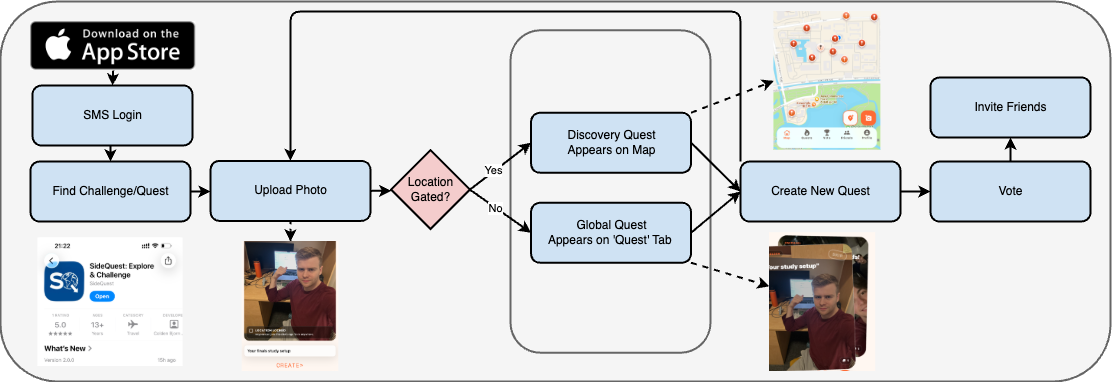
\includegraphics[width=0.85\textwidth]{ux-flow.png}
  \caption[User Flow Diagram]{User flow core loop.}
  \label{fig:ux-flow}
\end{figure}

\section{Participation Over Passive Social Media}
SideQuest was designed to encourage active participation rather than passive consumption. The app should make users feel curious about what is nearby and motivated to contribute something of their own. Voting has hourly caps to keep users from passively swiping and encourage them to interact with their environment. Additionally, SideQuest uses pairwise comparisons instead of `likes'. The chess-inspired voting creates a more game-like interaction and helps surface strong submissions, all while avoiding the popularity dynamics of simple like/dislike systems. Importantly, SideQuest voting gives users a taste of what Quests are available on the platform without devolving into a toxic consumption loop. The experience should feel more like participating in a shared adventure than posting into a generic social feed.

\section{Preserving Discovery}
Discovery is precious. It wouldn't feel special if a user already knew everything about a place before they went there. SideQuest protects the experience of discovery by only showing map markers and challenge prompts until a user is physically present in the location themselves. This allows users to discover areas themselves, with SideQuest only providing a small hint. Similarly, some places are personally meaningful. SideQuest respects users' decisions about what to share, allowing private friend-only Quests.

\section{Guiding Design Principles}
There are five guiding design principles that inform the design of SideQuest.

\subsection{Less is More}
The user interface should emphasize the core loop and avoid unnecessary clutter. SideQuest is image-first and interaction-first, so the design should prioritize photos, maps, and gestures rather than long blocks of text.

\subsection{Clear Affordances}
The interface should signal how it is meant to be used. Layered cards should feel swipeable. Map markers should feel tappable. Blocked/incomplete user actions should be clearly explained. Users should not have to guess what a screen is for or if their submission went through. 

\subsection{Do Not Make the User Wait}
One of the most important product goals is responsiveness. Waiting breaks the feeling of exploration and play, so the app should avoid unnecessary delay wherever possible. This principle later justifies caching, prefetching, optimistic uploads, and queued voting.

\subsection{Creativity Through Constraint}
Quests are structured rather than open-ended. This constraint is intentional. It gives users a prompt, makes places feel distinct, and creates a stronger basis
for competition rather than unstructured posting. Voting is capped to push users to create or explore rather than consume.

\subsection{Design for Delight, Not Everyone}
Rather than chase mass appeal from the beginning, SideQuest's design is tailored for a specific type of user who enjoys discovery, adventure, playful-sharing, and competition. The goal is not to become a universal social platform immediately, but to create an experience that feels memorable for the people it fits best.

\section{Evolving the Concept Through User Behavior}
Although the original model was one challenge, one location, many photos, user behavior showed that some kinds of participation did not fit neatly into a fully location-locked structure. Users wanted to post similar ideas from different places, compete with friends in different locations, and create broader thematic prompts. In response, SideQuest introduced non-location-locked Quests while keeping geo-locking as the default. This preserved the original emphasis on place-based discovery while allowing the system to support a wider range of social and creative use cases.

% ============================================================================
\chapter{System Architecture}
\label{ch:system}

SideQuest uses a client-server architecture with split storage. The mobile client is optimized for responsiveness in map and photo-heavy views, while the server remains authoritative for Quest visibility, matchmaking, ranking, and vote recording. Images are stored separately from application records, and a small set of runtime mechanisms keeps interactions fast without moving trust away from the backend. This chapter describes the system components, the persistent data model, and the runtime mechanisms that support low-latency interaction.

% architecture figure
\begin{figure}[!htbp]
  \centering
  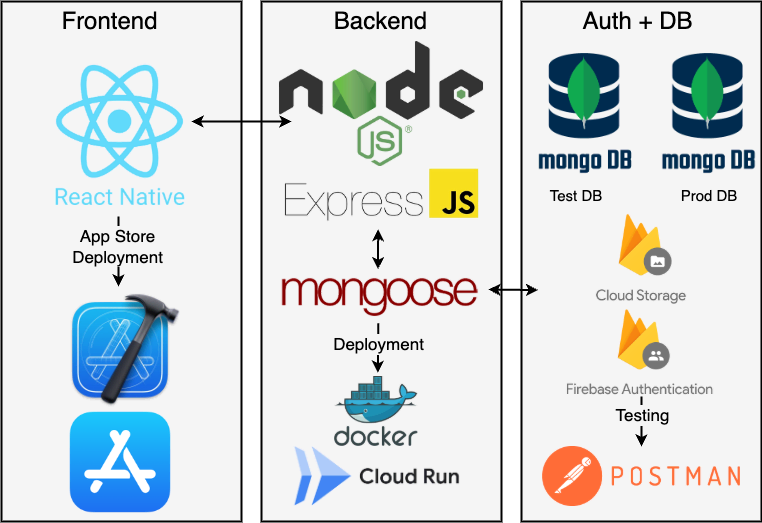
\includegraphics[width=0.6\linewidth]{arch-diagram.png}
  \caption[System Architecture Diagram]{Overview of the SideQuest architecture. The client handles presentation and responsiveness, while the server owns application state and rule enforcement.}
  \label{fig:architecture}
\end{figure}

\section{Application Architecture}

SideQuest is implemented as a full-stack mobile system. The user-facing application is built in React Native with Expo, the API service is implemented in Node.js and Express, MongoDB stores structured application data, and Firebase provides authentication and image storage. This structure keeps the system simple while separating interaction logic, application records, and media files.

\subsection*{Mobile Client}

The mobile client renders the main user experience: the map, Quest pages, upload flow, voting screens, and profiles. Its architectural role is responsiveness. It manages navigation, device capabilities such as camera and location, local caches, and image prefetching so that screens can appear quickly even when network requests are still in progress.

This creates the main split in the system: the client is responsible for presentation speed, while the server is responsible for correctness. That division is especially important in SideQuest because the app is image-heavy and users move frequently between the map, Quest pages, and duel views.

Figure~\ref{fig:navigation_graph} summarizes the main navigation structure implemented with Expo Router.

\begin{figure}[!htbp]
  \centering
  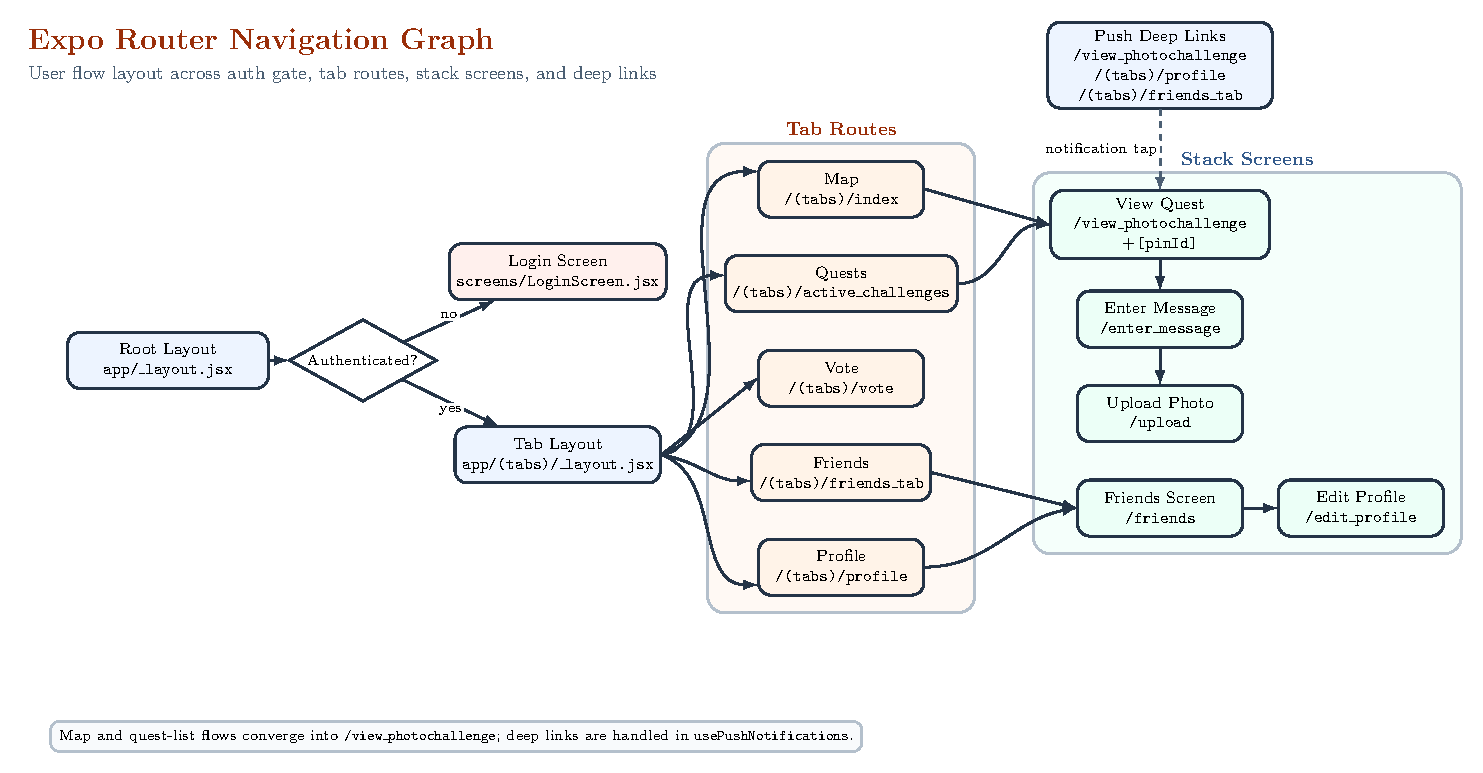
\includegraphics[width=0.95\linewidth]{08_navigation_graph.pdf}
  \caption[Navigation Graph]{Navigation graph for the main Expo Router structure.}
  \label{fig:navigation_graph}
\end{figure}

\subsection*{API Service}

The backend exposes a REST-style API used by the mobile client. It handles Quest creation, photo submission, Quest retrieval, friendship state, duel generation, and vote submission. More importantly, it is the system authority for state transitions. Permission checks, private Quest visibility, Elo updates, hourly vote limits, and duel validation are all enforced on the server.

This design keeps trust boundaries clear. The client can preload content and optimize presentation, but it cannot decide which votes are valid or how rankings change. That makes the interface feel immediate without giving up server control over competitive interactions.

\subsection*{Persistence and Platform Services}

MongoDB stores the application's structured records, including Quests, photo submissions, profiles, friendships, and vote history. Firebase provides two external services that are better kept outside the main API: user authentication and image storage. In practice, this means SideQuest stores metadata in MongoDB and stores uploaded photos in Firebase Storage, referenced by URL.

This split is a practical trade-off. MongoDB handles flexible application records well, while Firebase removes the need to build custom identity and media infrastructure. As a result, the backend can remain focused on domain logic rather than binary storage or credential management.

Figure~\ref{fig:create_challenge_sequence} shows the main write path for creating a Quest.

\begin{figure}[!htbp]
  \centering
  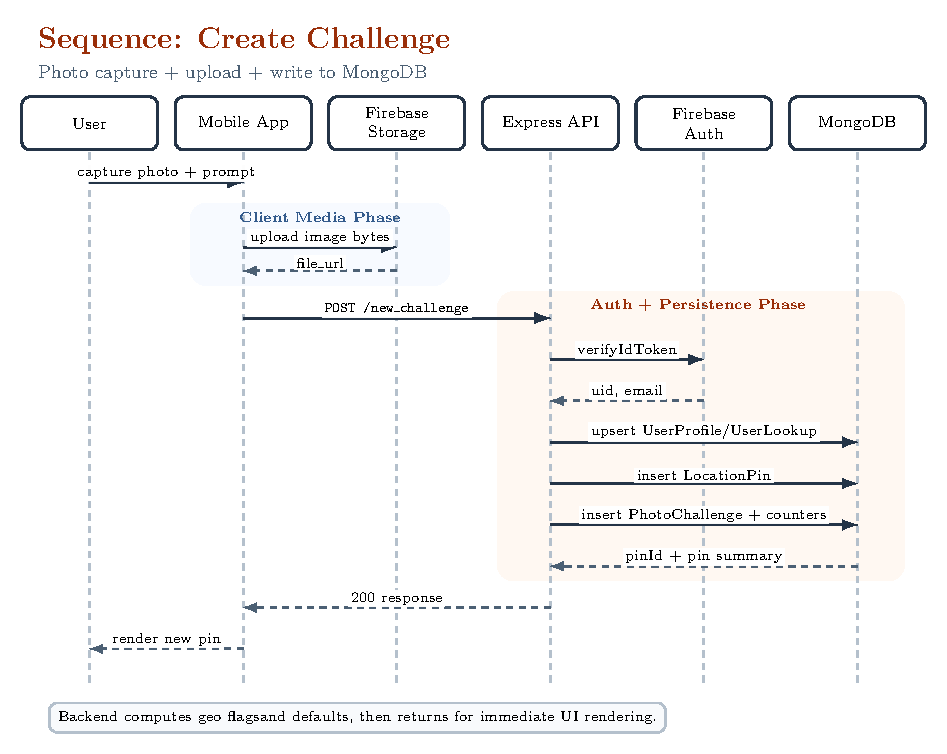
\includegraphics[width=0.9\linewidth]{03_sequence_create_challenge.pdf}
  \caption[Create Quest Flow Diagram]{Sequence diagram for the Quest creation flow.}
  \label{fig:create_challenge_sequence}
\end{figure}

\section{Data Architecture}

The data model is organized around the system's main write path: create a Quest, attach photos to that Quest, and record pairwise votes on those photos. Four records carry most of that flow: \texttt{UserProfile}, \texttt{LocationPin}, \texttt{PhotoChallenge}, and vote events. Supporting collections such as friendships, saved quests, and notification logs extend the system around that core.

Most relationships are reference-based. Pins store their creator, photos store both their parent pin and creator, and vote records store the winning and losing photos. This keeps writes simple and avoids large embedded documents that would be expensive to update as activity grows.

The main read path is more denormalized than the write path. Pins cache fields such as photo count, recent image URL, and top-ranked photo. Photos store local and global Elo scores, win/loss counts, and a visibility bucket used for matchmaking. User profiles keep lightweight counters for profile views. These values are updated during writes so that common reads such as map rendering, Quest loading, and profile summaries do not require repeated aggregation queries.

% data model figure
\begin{figure}[!htbp]
\centering
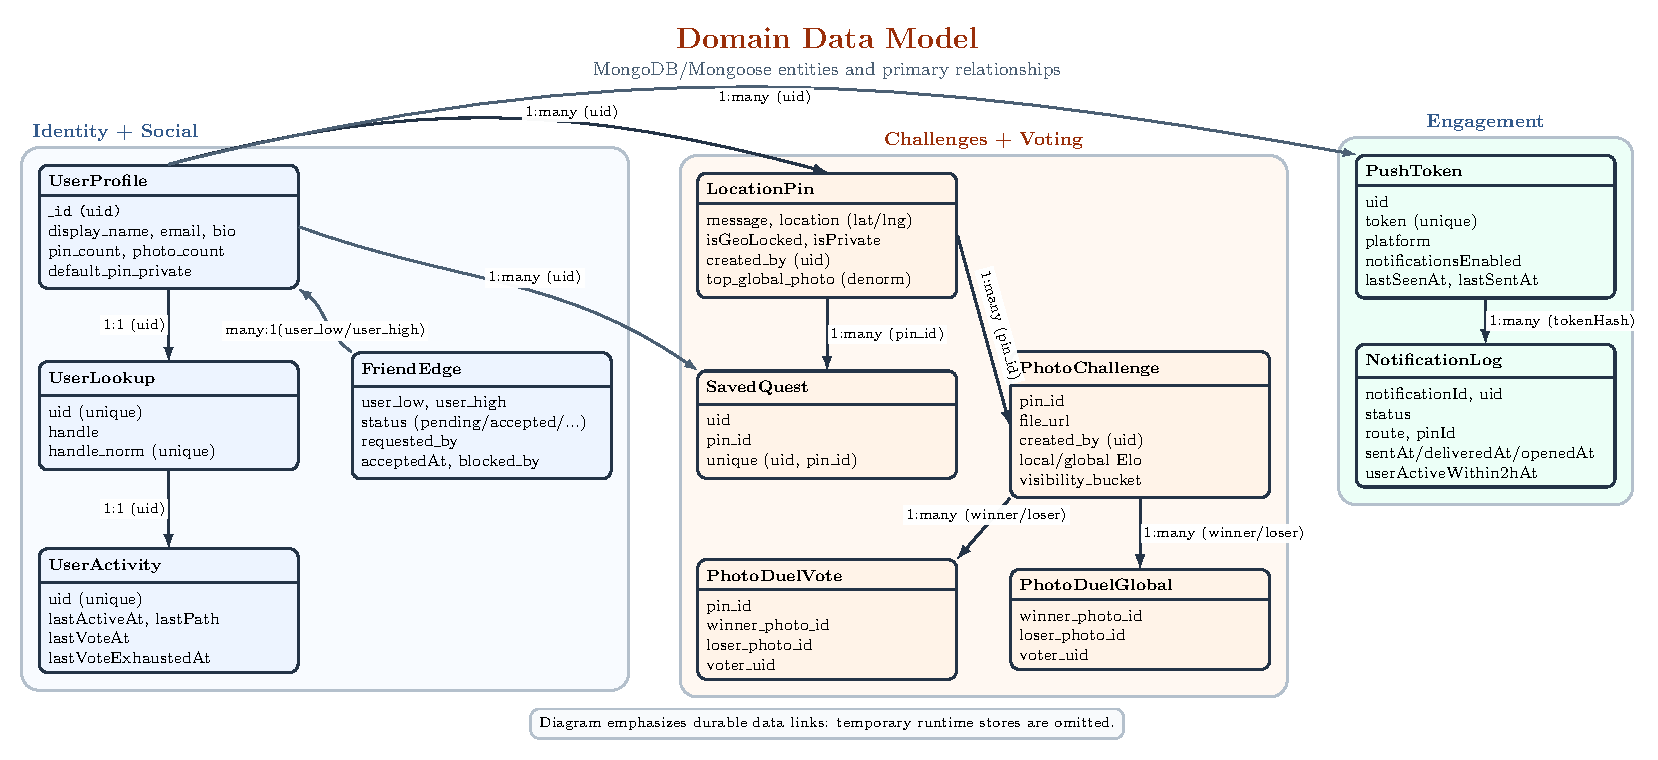
\includegraphics[width=0.9\textwidth]{01_domain_data_model.pdf}
\caption[Data Model Relationship Diagram]{Data model showing the main persistent relationships in MongoDB.}
\label{fig:data_design}
\end{figure}

\section{Runtime Mechanisms}

The persistent schema defines what the system stores. The runtime mechanisms define how the system feels. In SideQuest, these mechanisms exist for two reasons: to keep image-heavy interactions fast and to keep voting server-authoritative.

\subsection*{Cached Reads and Hydration}

Quest pages and profile views use a render-first caching strategy. When possible, the client shows cached metadata and photo lists immediately, then refreshes them in the background. Friends, friend requests, statistics, and top photos follow the same pattern. This reduces waiting time on frequently revisited screens.

The client also prefetches likely next images for duel cards, Quest photo galleries, and profile views. This matters because the app is visually dense: even when text data is small, image latency can dominate the interaction.

\subsection*{Duel Staging for Latency}

The vote screen avoids loading each duel from scratch. Instead, the client keeps a small queue of preloaded duel pairs so that advancing to the next comparison is nearly immediate. In parallel, the server maintains a short-lived per-user bucket of staged global duel pairs and replenishes it in the background. This reduces visible delay while still letting the backend control pair selection and hourly vote limits.

\subsection*{Vote Tokens for Integrity}

Each duel issued by the server includes a short-lived vote token bound to the user, duel scope, and photo pair. When the client submits a vote, the server validates and consumes that token before recording the result. This prevents replayed votes and ensures that the submitted vote matches a duel the server actually served.

Figure~\ref{fig:vote_token_sequence} highlights this flow.

\begin{figure}[!htbp]
  \centering
  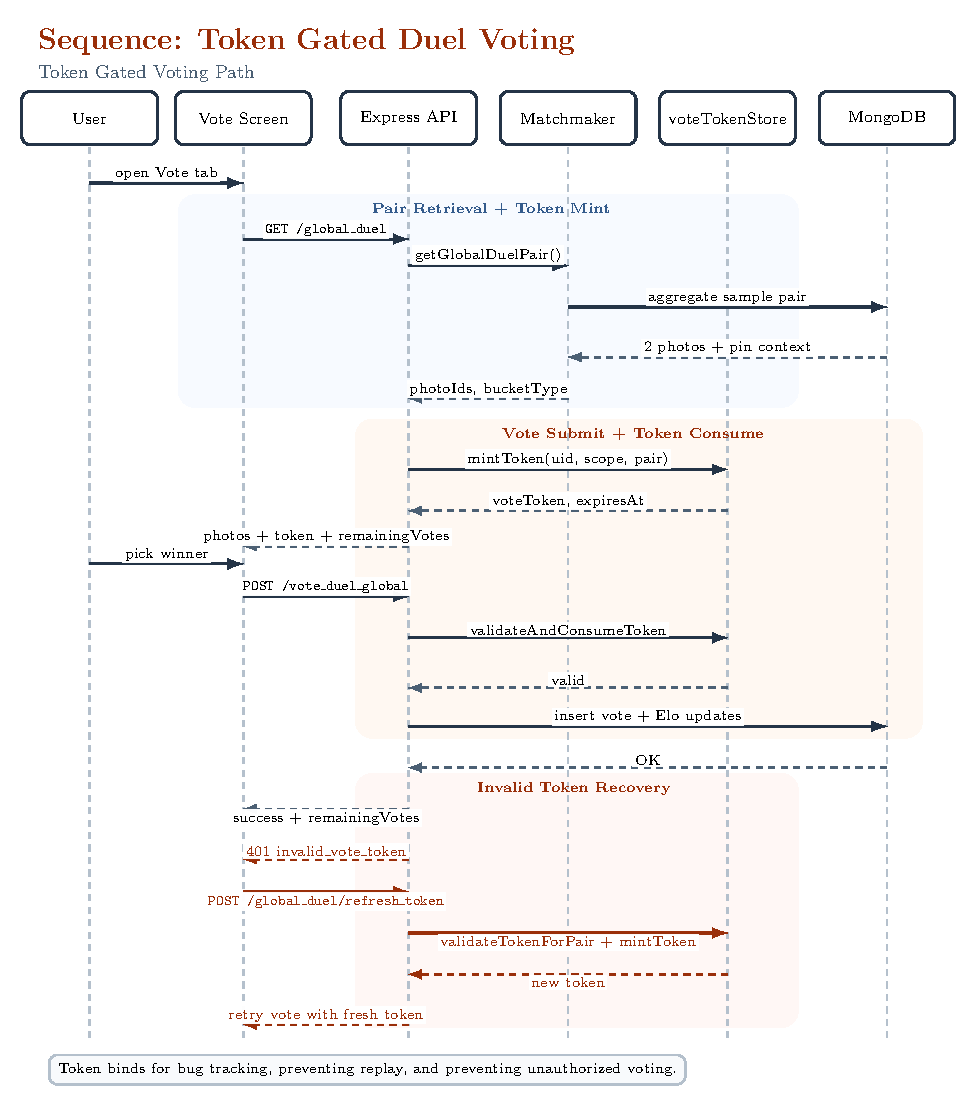
\includegraphics[width=0.95\textwidth]{04_sequence_global_duel_vote_token.pdf}
  \caption[Vote Token Flow Diagram]{Sequence diagram for duel issuance, token validation, and vote submission.}
  \label{fig:vote_token_sequence}
\end{figure}

\subsection*{Ranking and Matchmaking}

SideQuest uses two Elo scores per photo. Local Elo ranks submissions within a single Quest. Global Elo ranks photos across the whole platform. This allows the system to support both place-specific competition and cross-platform comparison.

Global duel selection is weighted rather than purely random. Some duels compare photos from the same Quest, preserving the meaning of the original prompt. Others draw from Elo-based visibility groups, which helps mix established and still-calibrating content. Quest-local matchups are also biased toward recent activity so newer Quests can enter circulation. Together, these rules balance freshness, fairness, and variety.

Detailed equations for Elo ranking and duel selection can be found in Appendix~\ref{sec:ranking}.

\subsection*{Geographic Handling}

A small region-specific mechanism affects map display in mainland China. When needed, stored coordinates are transformed before rendering so that map markers align with the local mapping standard (GCJ-02). This logic is kept separate from the main content model so that the rest of the system remains unchanged.

Taken together, these runtime mechanisms show the main architectural idea behind SideQuest: the client is optimized for responsiveness, but the server remains authoritative for competitive state. Cached reads, staged duels, and image prefetching make the app feel immediate, while server-side validation, matchmaking, and ranking keep the system consistent and fair.

% ============================================================================

\chapter{Development Process}
\label{ch:development}

SideQuest was developed through an iterative process that combined rapid prototyping, real user feedback, and frequent deployment. Rather than following a rigid engineering plan from the beginning, the project evolved through short development cycles in which new ideas were implemented, tested, and refined. This chapter describes how features were developed, how code was deployed, and how tools such as version control, automation, and AI-assisted programming supported the development process.

\section{Development Workflow}

The development of SideQuest followed an Agile-inspired workflow focused on rapid iteration and experimentation. Agile development emphasizes building small pieces of functionality, testing them quickly, and adjusting the product based on feedback. This philosophy fit the goals of the project well, since many aspects of the app—such as voting mechanics, challenge structure, and user interaction patterns—could only be evaluated once real people began using the system.

\begin{wrapfigure}{r}{0.38\textwidth}
\vspace{-6pt}
\centering
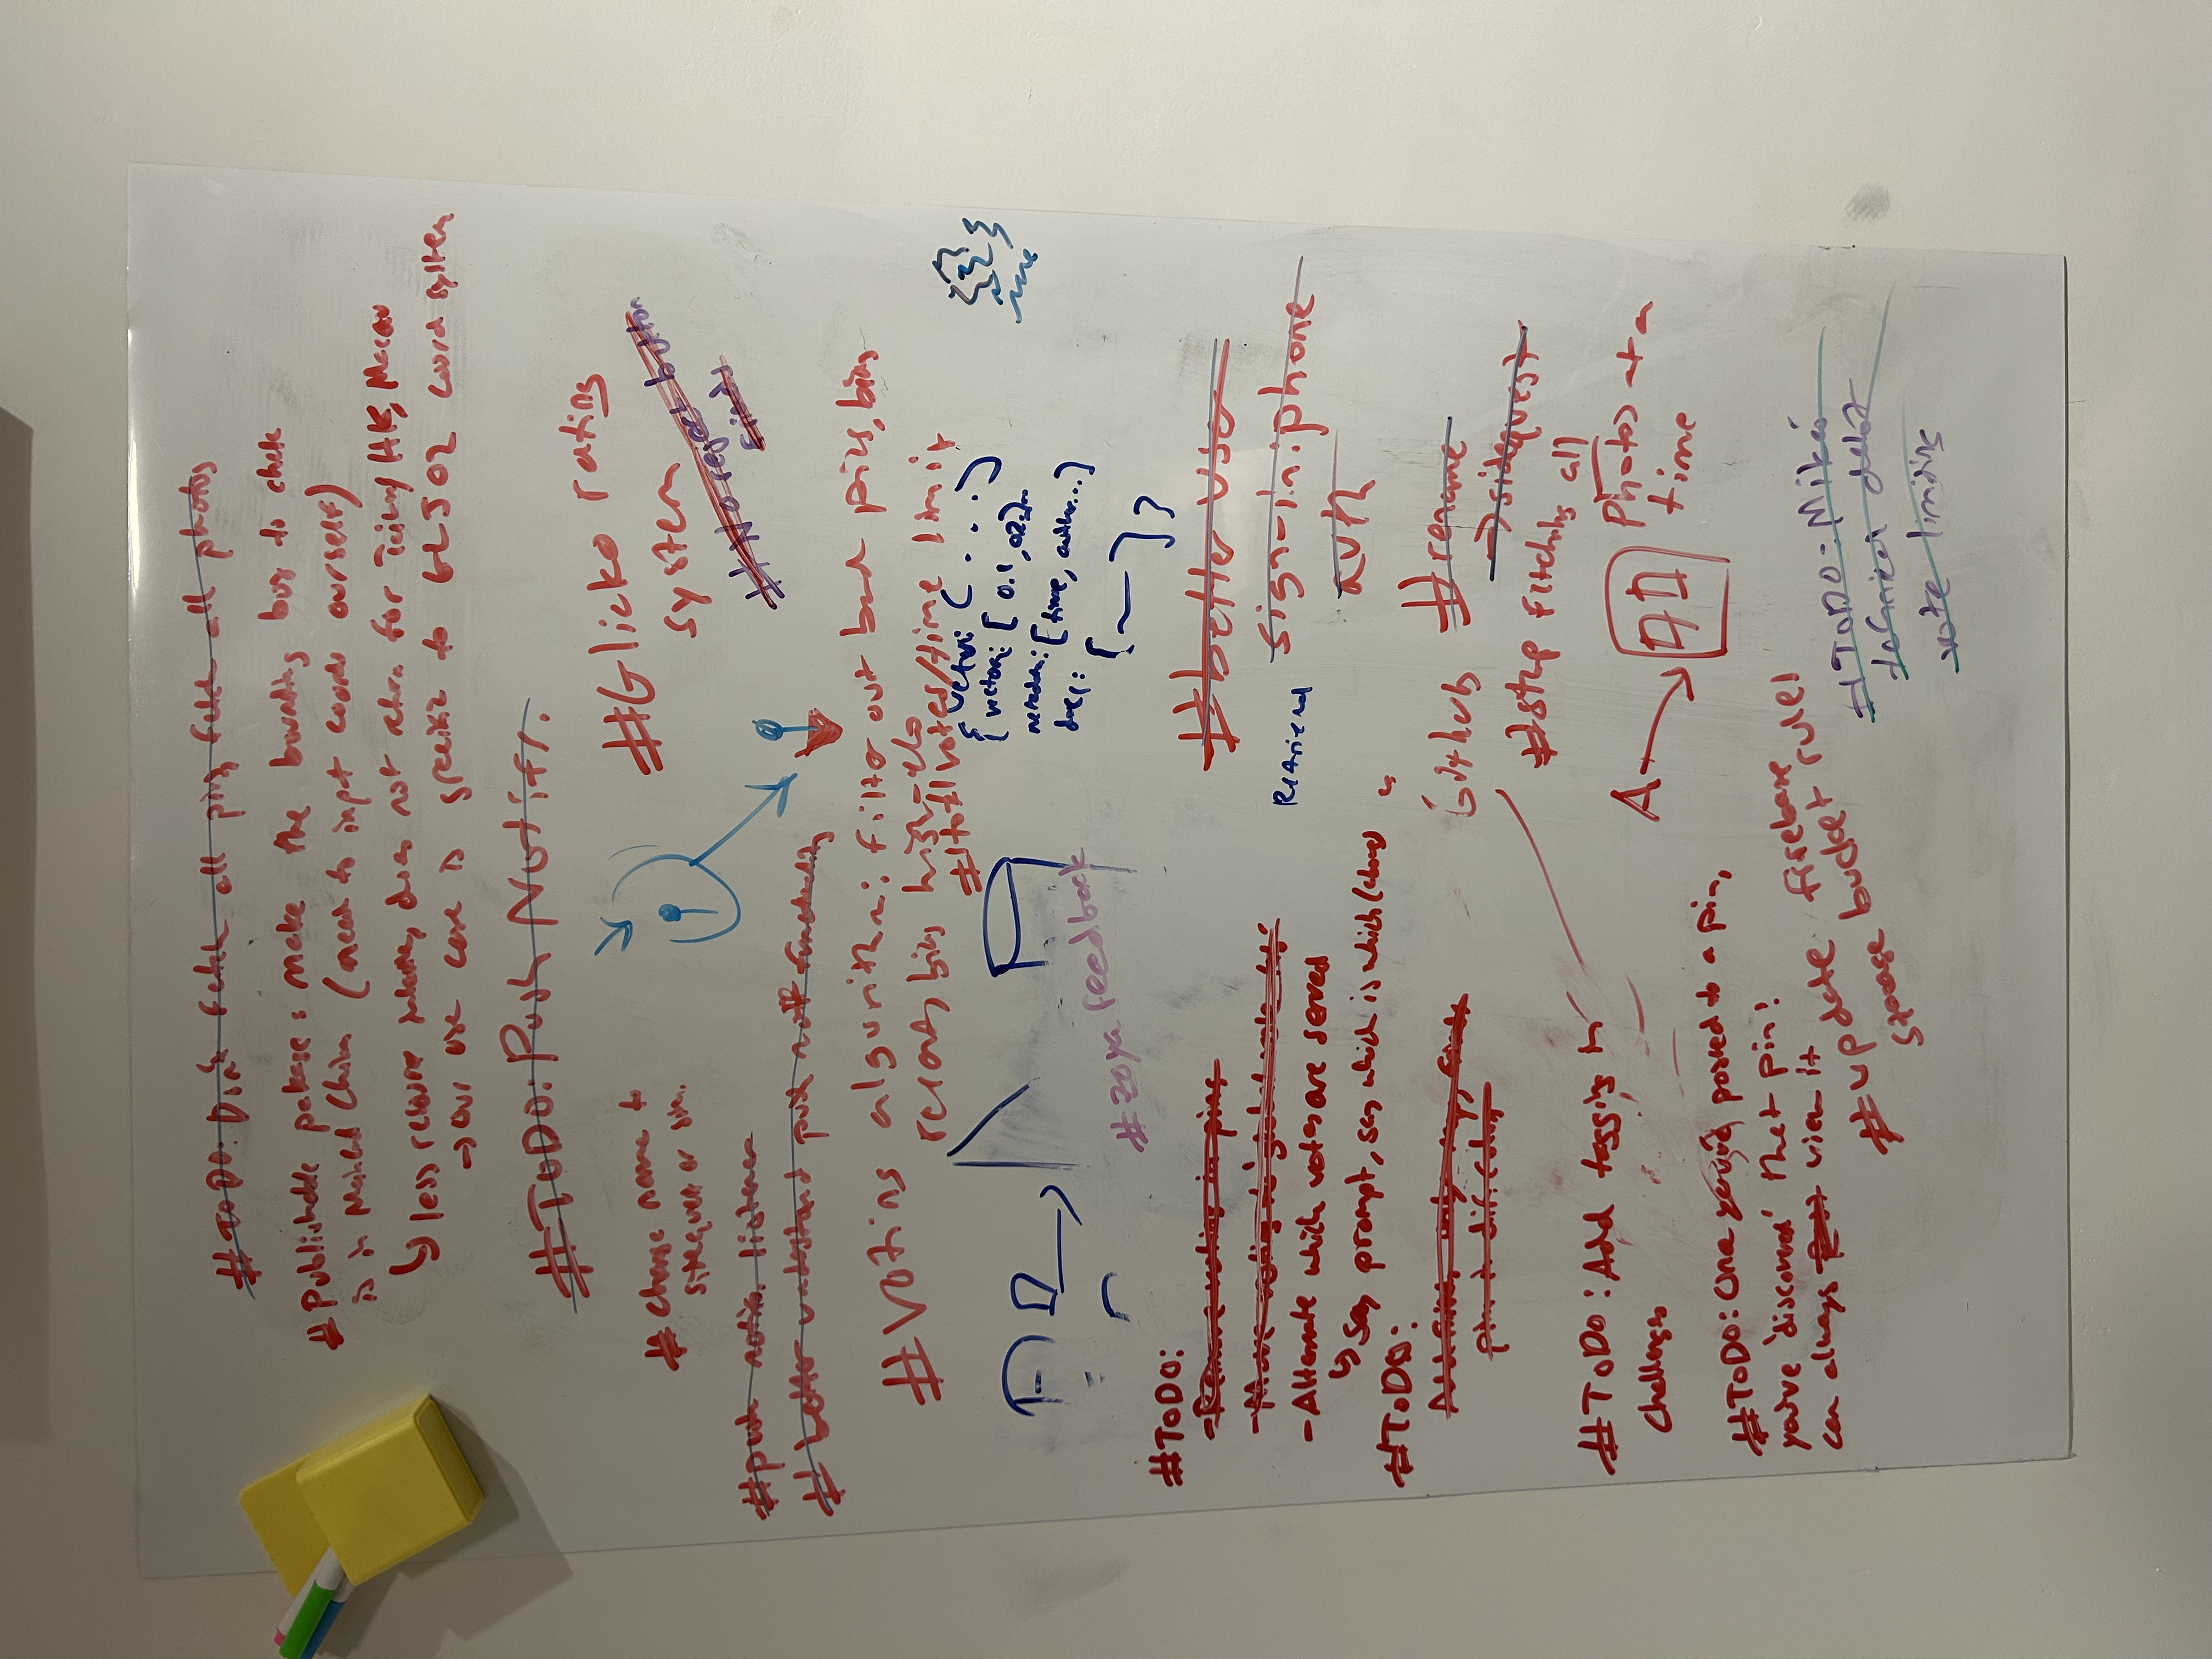
\includegraphics[width=\linewidth,angle=-90]{feedback-wall.jpeg}
\caption[User Feedback Backlog]{Photo of the user feedback backlog board.}
\label{fig:feedback_backlog}
\vspace{-6pt}
\end{wrapfigure}

Although the project did not formally implement Scrum, its workflow resembled a simplified version of that process. Development moved in roughly one‑week cycles that functioned like short sprints. At the beginning of each cycle, potential features and fixes were discussed and written onto a shared whiteboard backlog. These items were prioritized based on two factors: how much they would move the product closer to a functional and coherent experience, and how strongly they addressed feedback from users who had already tested the app.

Once a feature was selected, the design phase was usually brief. Many design decisions were discussed collaboratively between the two developers, sometimes supplemented by quick sketches or conversations with AI tools to explore implementation ideas. The goal was not to finalize a perfect design upfront but to produce a minimal version that could be tested quickly.

Most development time was spent in a tight loop of writing code, running the application, and testing new behavior on a physical device. Because SideQuest relies heavily on maps, camera input, and gesture interactions, testing directly on phones was often more reliable than using simulators alone. In some cases, automated unit tests written with Jest were used to verify specific logic, but most validation occurred through direct interaction with the working application.

Once a feature behaved correctly in basic tests, the changes were committed to Git and pushed to the project’s GitHub repository. Instead of grouping entire features into single commits, commits were kept relatively small and incremental. This approach made it easier to track changes, isolate bugs, and revert individual pieces of work if necessary. Over the course of a typical week‑long cycle, this process resulted in roughly three to five completed features or improvements.

\begin{figure}[!htbp]
  \centering
  \definecolor{sqorange}{HTML}{FF6B35}
  \definecolor{sqcoral}{HTML}{FFD9CC}
  \definecolor{sqpeach}{HTML}{FFE9D6}
  \definecolor{sqmint}{HTML}{DDF3E4}
  \definecolor{sqsky}{HTML}{DCEEFE}
  \definecolor{sqlav}{HTML}{E9E2FF}
  \definecolor{sqnotea}{HTML}{FFF4EE}
  \definecolor{sqnoteb}{HTML}{EEF7FF}

  \resizebox{\linewidth}{!}{%
  \begin{tikzpicture}[
    font=\sffamily,
    box/.style={draw=sqorange!80!black, text=black, rounded corners=6pt, minimum width=34mm, minimum height=12mm, align=center, line width=0.45pt},
    note/.style={draw=sqorange!65!black, rounded corners=6pt, inner xsep=6pt, inner ysep=4pt, align=left, line width=0.4pt},
    arrow/.style={-Latex, thick, draw=sqorange!85!black},
    node distance=14mm
  ]

  \node[box, fill=sqcoral] (design) {Design};
  \node[box, fill=sqpeach, right=of design] (dev) {Development};
  \node[box, fill=sqmint, right=of dev] (test) {Testing};
  \node[box, fill=sqsky, right=of test] (deploy) {Deployment};
  \node[box, fill=sqlav, right=of deploy] (feedback) {User Testing};

  \draw[arrow] (design) -- (dev);
  \draw[arrow] (dev) -- (test);
  \draw[arrow] (test) -- (deploy);
  \draw[arrow] (deploy) -- (feedback);

  \draw[arrow] (feedback.south) .. controls +(0,-14mm) and +(0,-14mm) .. (design.south);

  \node[draw=sqorange!70!black, dashed, rounded corners=10pt, fit=(design)(dev)(test)(deploy)(feedback), inner sep=9mm] (sprint) {};
  \node[fill=white, text=sqorange!85!black, inner sep=2pt, font=\bfseries\small] at ([yshift=7mm]sprint.north) {1-week Sprint (repeat weekly)};

  \node[note, fill=sqnoteb, below=20mm of feedback, anchor=north] (backlog) {\textbf{User Stories $\rightarrow$ Backlog}\\
  \footnotesize
  \begin{tabular}{@{}l@{}}
  - Convert feedback into user stories \\
  - Add stories to the whiteboard backlog \\
  - Prioritize fixes + next features
  \end{tabular}};
  \draw[arrow] (feedback.south) -- ++(0,-6mm) -- (backlog.north);

  \end{tikzpicture}%
  }
  \caption[Agile Workflow Diagram]{Agile-inspired workflow.}
  \label{fig:agile-cycle}
\end{figure}

Git played a central role in coordinating development and maintaining stability. Because both developers worked on separate machines, version control allowed work to proceed in parallel while preserving a shared history of the codebase. Commit history also served as an effective debugging tool: when a bug appeared, recent changes could be inspected to identify which modification introduced the issue. In many cases, reverting or adjusting a small number of commits was enough to restore correct behavior.

\section{Deployment}

Deploying new versions of SideQuest initially proved to be one of the most time‑consuming parts of development. The project contains two major components—the backend API and the mobile application—and each required its own build and deployment process. Differences between local development environments often caused builds to fail or behave inconsistently. Because each build attempt could take tens of minutes, debugging deployment issues frequently slowed development.

To solve this problem, the project adopted a continuous integration and continuous deployment (CI/CD) pipeline. CI/CD systems automatically build and deploy software whenever changes are pushed to a repository, ensuring that the same build process runs in a consistent environment every time.

The backend service is packaged as a Docker container. The container defines all required dependencies and startup commands, ensuring that the service runs identically regardless of the underlying machine. This container is deployed to Google Cloud Run, which automatically builds the container when new code is pushed to GitHub and replaces the previous version with the updated service.

The mobile application follows a different deployment path. React Native code must ultimately be compiled into a native iOS application before it can be distributed. This process uses Apple’s Xcode build tools and is integrated with Xcode Cloud for automated builds. When the frontend repository receives new commits, Xcode Cloud installs the necessary dependencies, builds the iOS application, and prepares it for distribution through TestFlight or the App Store.

Although the cloud build process can take longer than a local build—particularly because SideQuest is not written in Apple’s native Swift language—the automated pipeline removes the need for manual deployment steps. More importantly, it guarantees that builds occur in a clean and consistent environment, eliminating many of the configuration issues that previously interrupted development.

\section{Role of AI in Development}

AI-assisted programming tools were used throughout the development of SideQuest. Systems such as OpenAI Codex, Anthropic Claude, and AI-enabled editors like Cursor were used to accelerate development, generate code scaffolding, and assist with debugging.

These tools proved particularly effective for implementing repetitive patterns, building user interface components, and integrating code with existing frameworks. In many cases, AI suggestions made it possible to prototype features significantly faster than writing every line manually.

However, AI systems also had clear limitations. They sometimes produced overly large code changes, introduced subtle errors, or struggled with complex multi-step features. As a result, AI output always required careful review and testing by the developers before being integrated into the codebase.

One especially useful workflow involved combining AI debugging with Git version control. When difficult bugs appeared, AI tools were sometimes used to add detailed logging throughout a feature. After reproducing the bug, the logs could be analyzed to identify the underlying problem. Once the issue was resolved, the additional logging could easily be removed by reverting the debugging commits in Git.

Overall, AI tools functioned less as replacements for developers and more as productivity accelerators. They reduced the time required to implement ideas and experiment with new features, while human developers remained responsible for system architecture, debugging, and design decisions.

% ============================================================================
%
\chapter{User Testing and Iteration}
\label{ch:testing}

User testing and iteration were central to how SideQuest developed over time. Rather than treating feedback as something collected only after features were finished, we used it throughout development to shape what the app became. That approach fits the broader Agile process behind the project. New ideas were discussed with potential users, translated into features, tested in working builds, and then revised based on what people actually did with the app.

This chapter looks at SideQuest through that process of iteration. It begins with the app's early state to establish what the first prototypes could and could not do. It then follows three features from initial conversations with users through implementation and later revision. Looking at the project this way gives a clearer picture of how user feedback influenced concrete design decisions, and it shows that the final product was not built all at once, but shaped gradually through repeated testing and refinement.

\section{Early State of the App}
The earliest version of SideQuest was built in under a month, in April 2025. At that stage, the app was extremely simple: users could upload photos to a map, where each upload appeared as a marker with its photo attached, and they could view basic account information in a profile section. Although this version lacked many of the features that define the app today, it worked as an important proof of concept. It established that the core interaction---exploring a map and engaging with location-based media---was compelling enough to build on further. Even now, the map remains the center of the SideQuest experience.

\begin{figure}[!htbp]
\centering

\begin{subfigure}{0.2\textwidth}
\centering
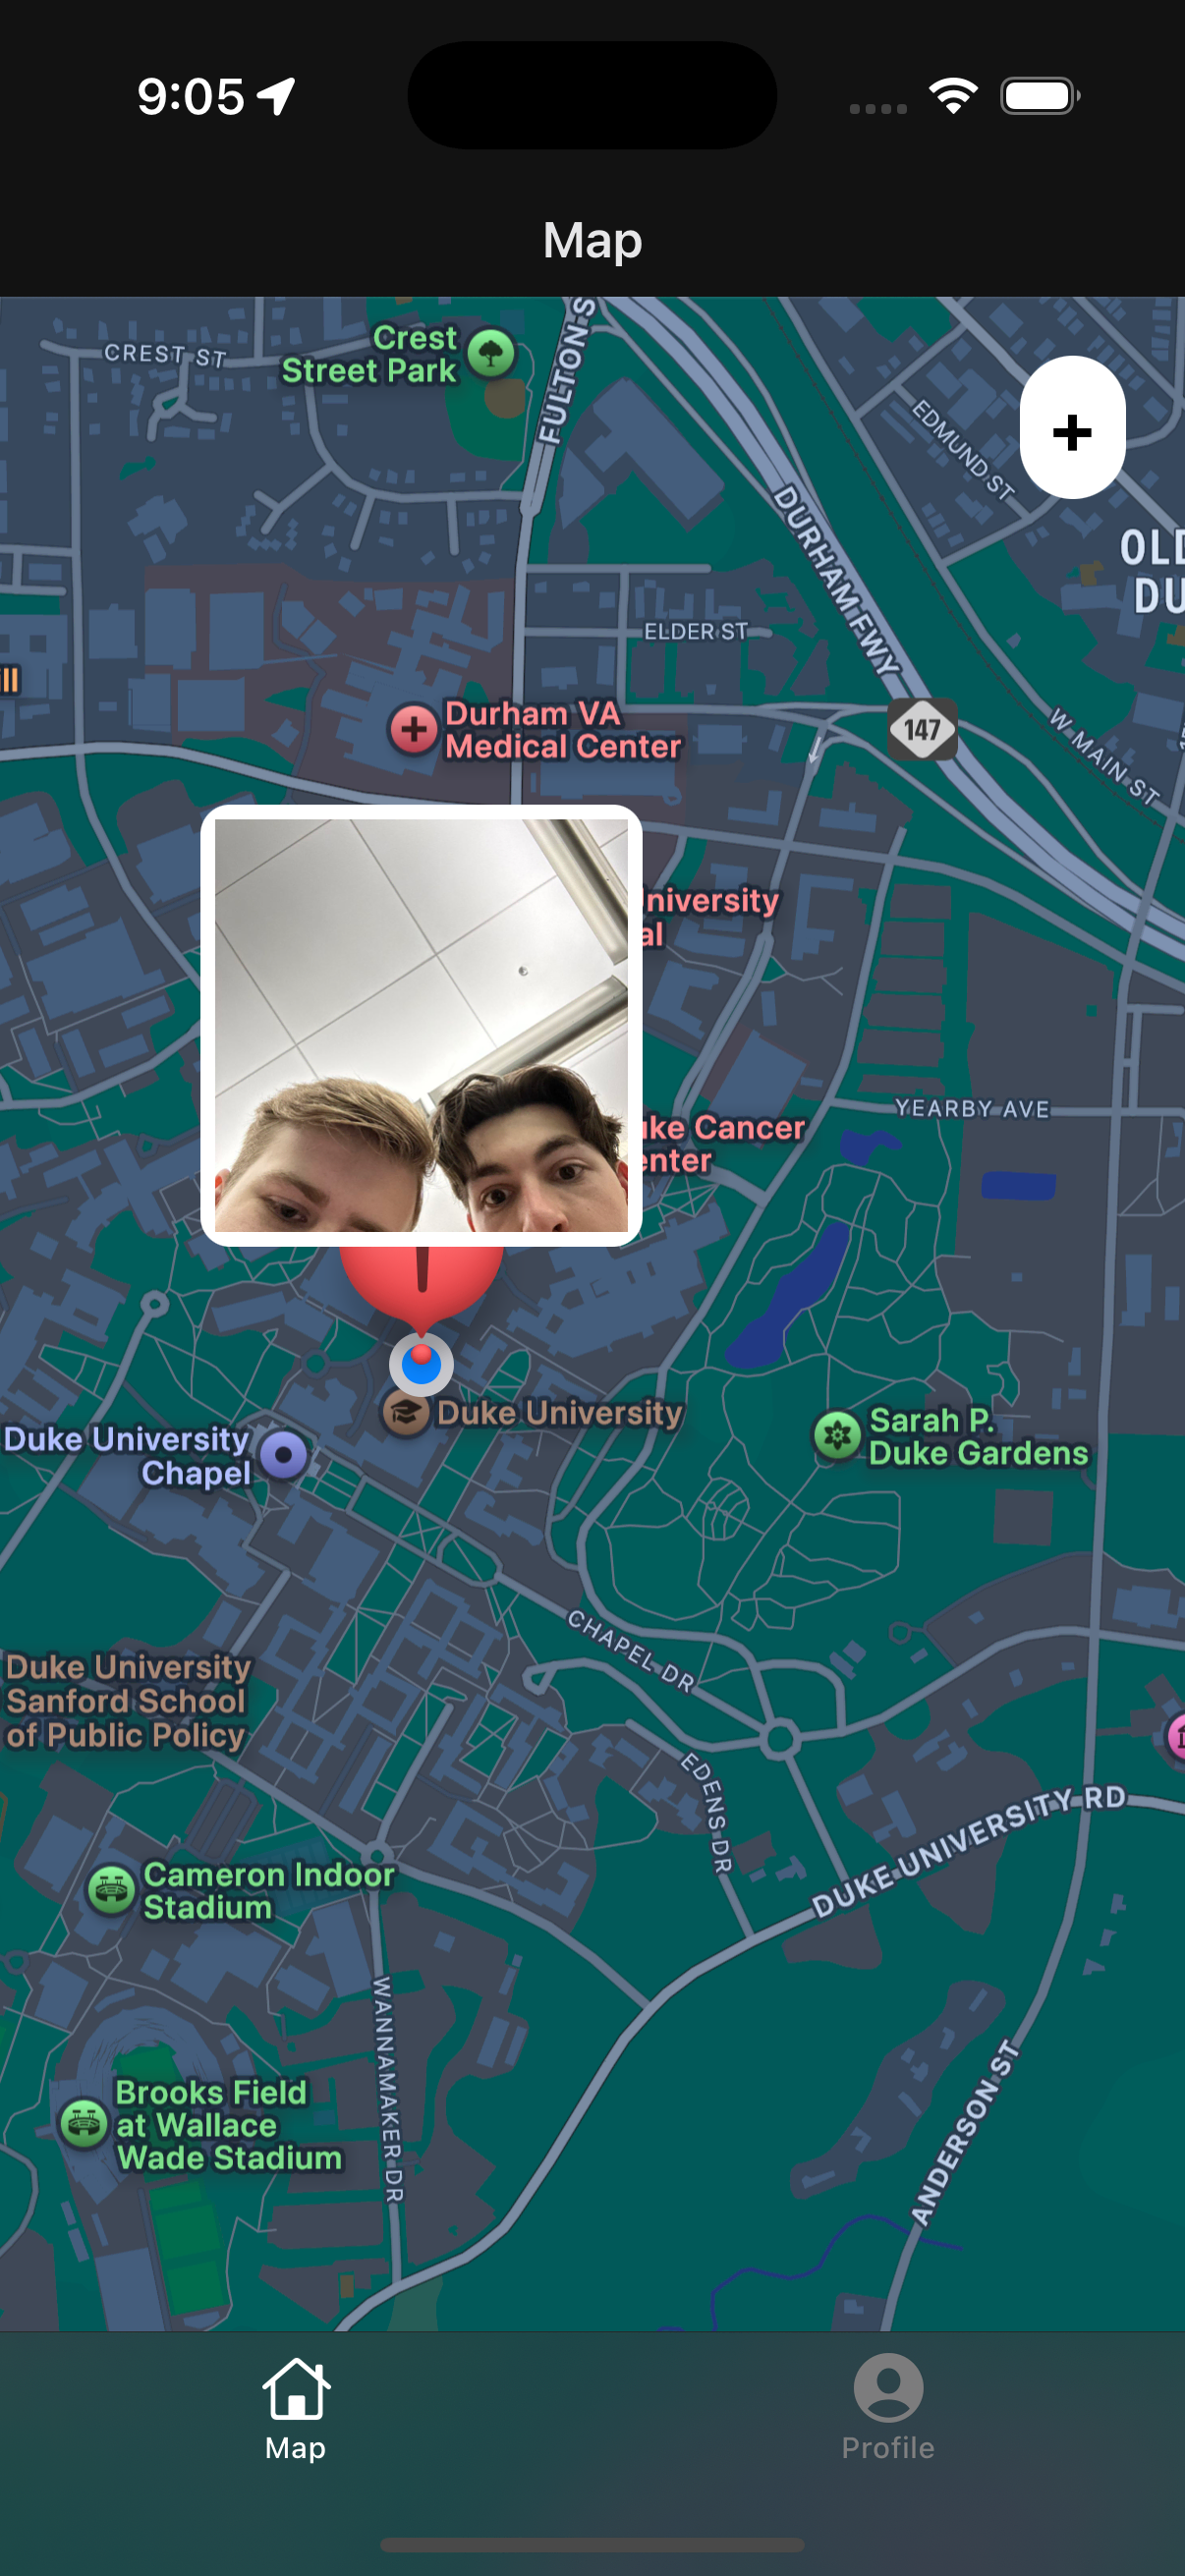
\includegraphics[width=\linewidth]{init_map.png}
\end{subfigure}
\hspace{2mm}
\begin{subfigure}{0.2\textwidth}
\centering
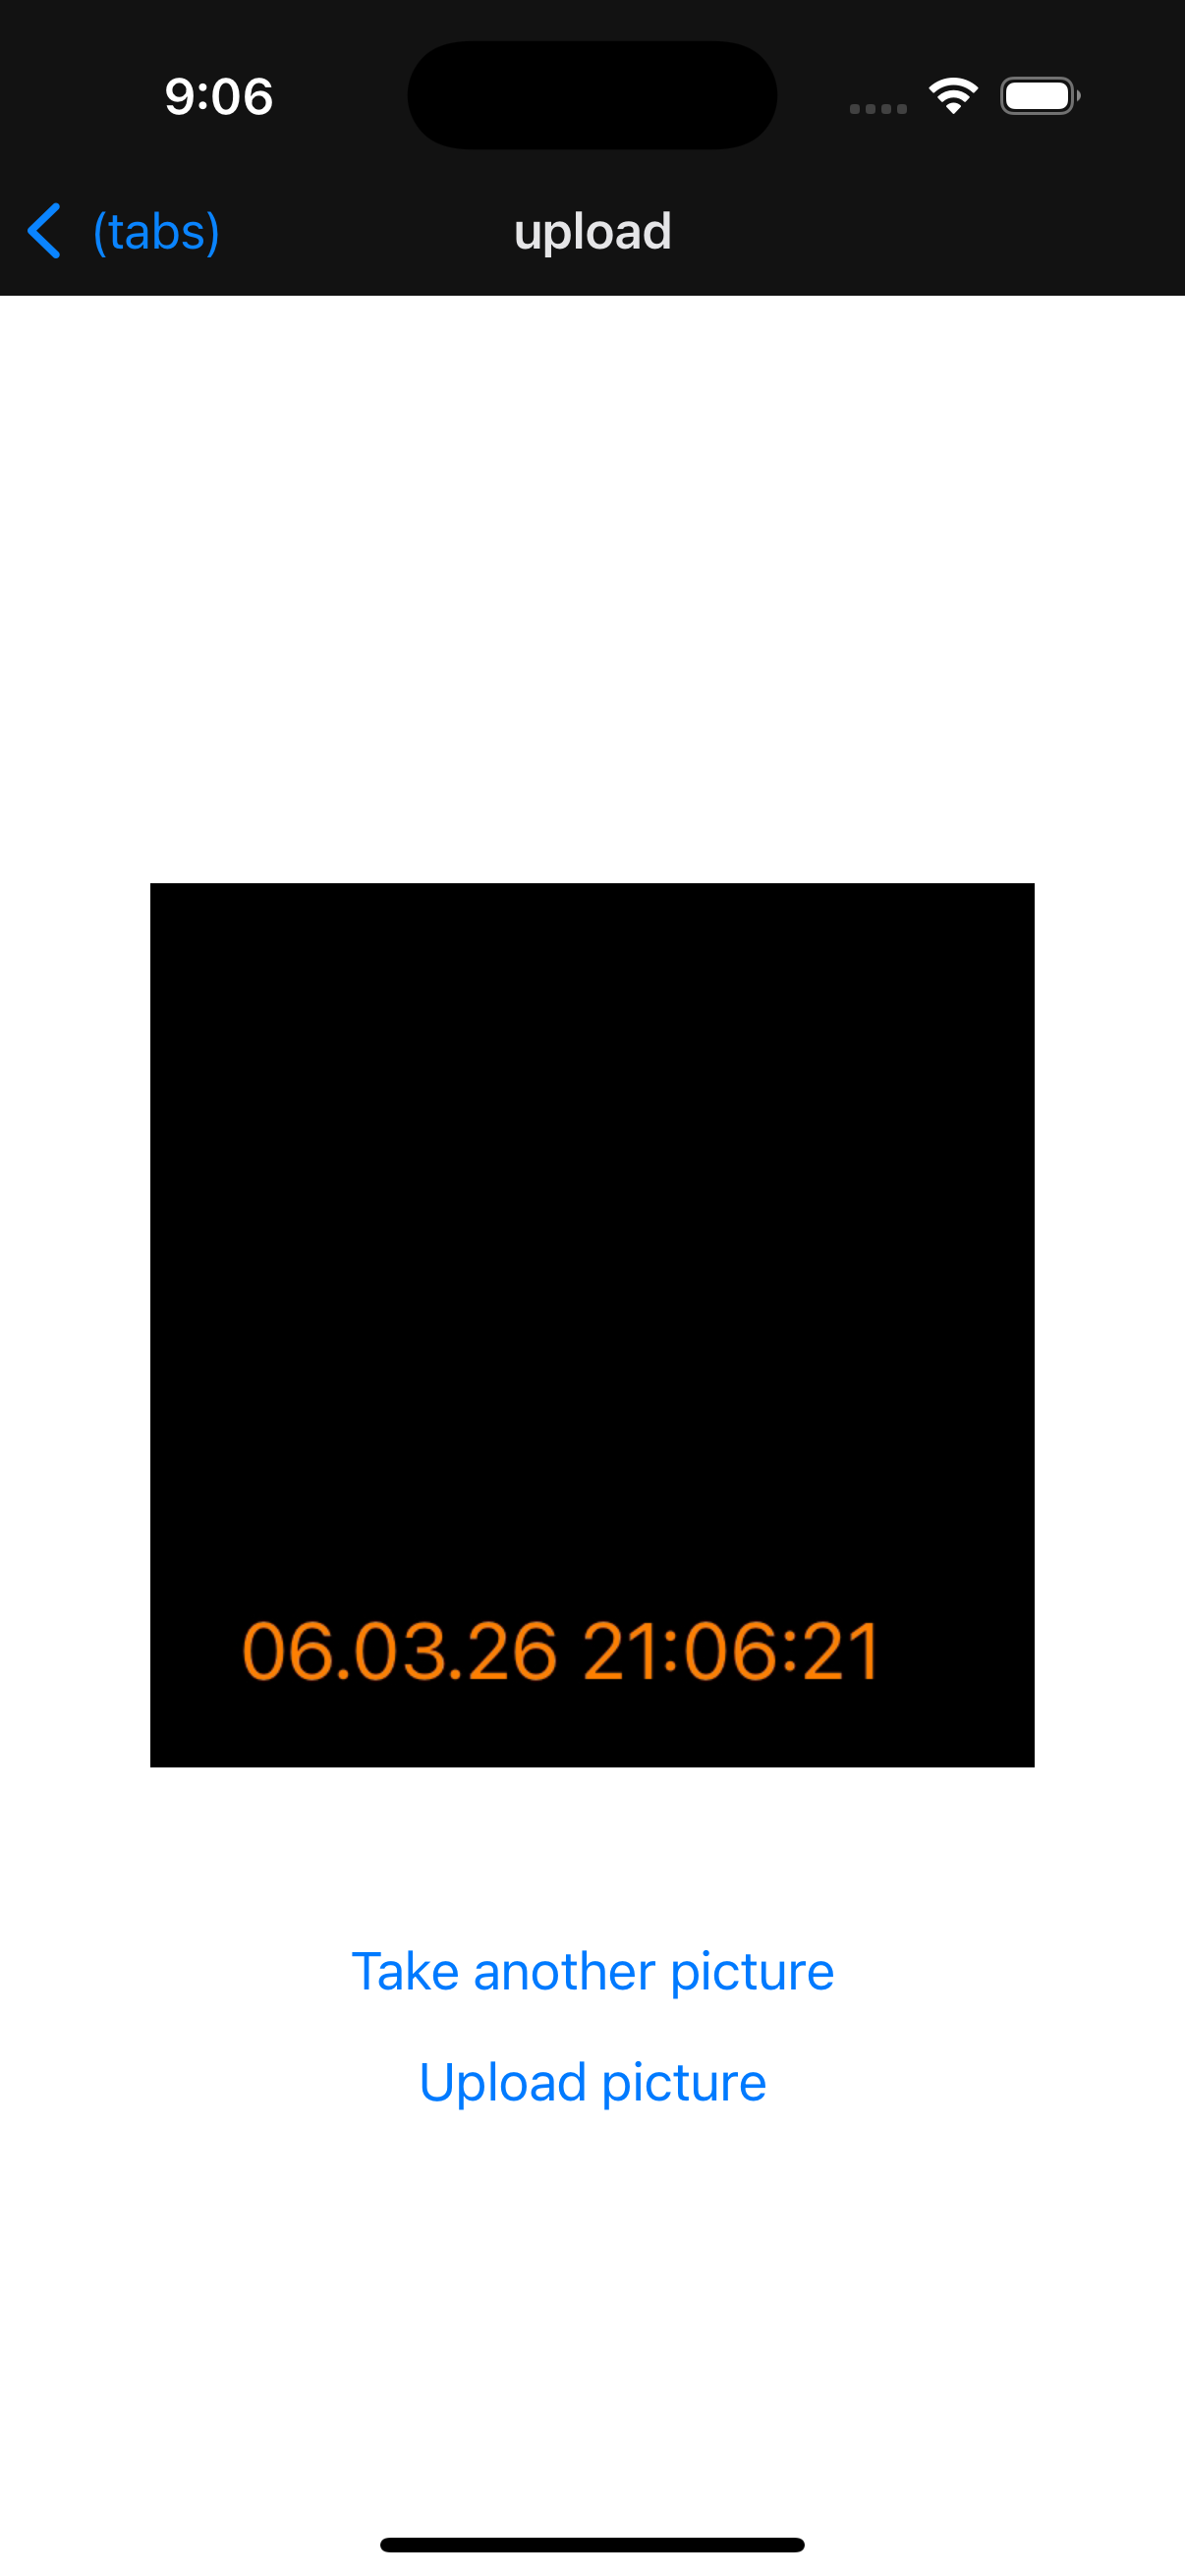
\includegraphics[width=\linewidth]{init_submit.png}
\end{subfigure}
\hspace{2mm}
\begin{subfigure}{0.2\textwidth}
\centering

\includegraphics[width=\linewidth]{init_profile.png}
\end{subfigure}

\caption{Screenshots showing the earliest stages of the map, Quest submission, and profile screens.}
\label{fig:inital_screens}
\end{figure}

After four more months of development, the structure of the app had become much closer to its current form. SideQuest now included dedicated map, vote, and profile tabs. The vote tab displayed two photos side by side and allowed users to tap one to declare it the winner. The data model had also become more sophisticated. Photos were no longer treated as standalone uploads; instead, they were separated from challenges. A single challenge, now a Quest, was tied to a real-world location and could now contain multiple photo submissions, while each photo belonged to only one Quest. This change made the app feel less like a map of isolated posts and more like a system built around place-based prompts and responses. Quests and their associated photos could both be viewed from the map, bringing the app closer to the experience it was ultimately trying to create.

\section{Iterations on Feedback}
For the rest of this chapter, the focus is on three features whose development best illustrates the role of user feedback in shaping SideQuest. In each case, the process followed a similar pattern: an initial need or frustration surfaced in conversation or testing, a feature was designed in response, and that feature was then revised again once people began using it in practice. Following these examples from early discussion to final implementation shows how iteration worked at the level of specific product decisions, rather than only at the level of general development philosophy.

\subsection{Feature One: Uploading a Photo}

\begin{figure}[!htbp]
\centering

\begin{subfigure}{0.3\textwidth}
\centering
\includegraphics[width=\linewidth]{pre_upload.PNG}
\end{subfigure}
\hspace{2mm}
\begin{subfigure}{0.3\textwidth}
\centering
\includegraphics[width=\linewidth]{post_upload.PNG}
\end{subfigure}

\caption{Screenshots showing the changes in the upload screen.}
\label{fig:upload_before_after}
\end{figure}

Initially, SideQuest kept users on the upload screen until a photo had fully uploaded. The upload button was greyed out while the image was processing, but that change was subtle enough that some users did not notice it. In one test, a user pressed the ``Upload'' button more than six times before commenting that it ``wasn't doing anything.'' This made it clear that the app was not giving enough feedback during what could feel like a stalled or uncertain moment.

To make the process feel more responsive, the upload flow was changed so that users were returned to the main screen immediately while the photo continued uploading in the background. That solved the problem of users feeling stuck on the upload page, but it introduced a new one. When shown this updated version, the same user repeated the flow and then asked, ``What happened to my photo?'' To address that confusion, a small toast message was added to confirm that the upload was in progress and later update the user on whether it had succeeded or failed. This iteration made the upload flow feel faster while still giving users enough feedback to trust that the app was working.

\subsection{Feature Two: Voting}
Voting is the feature that has gone through the most redesigns. When it was introduced originally, the idea was to use it as a way to give users a taste of what others were doing on SideQuest and give badges to users with the best photos. It also had the added benefit of weeding out photos that were low-effort. 

\begin{figure}[!htbp]
\centering

\begin{subfigure}{0.3\textwidth}
\centering
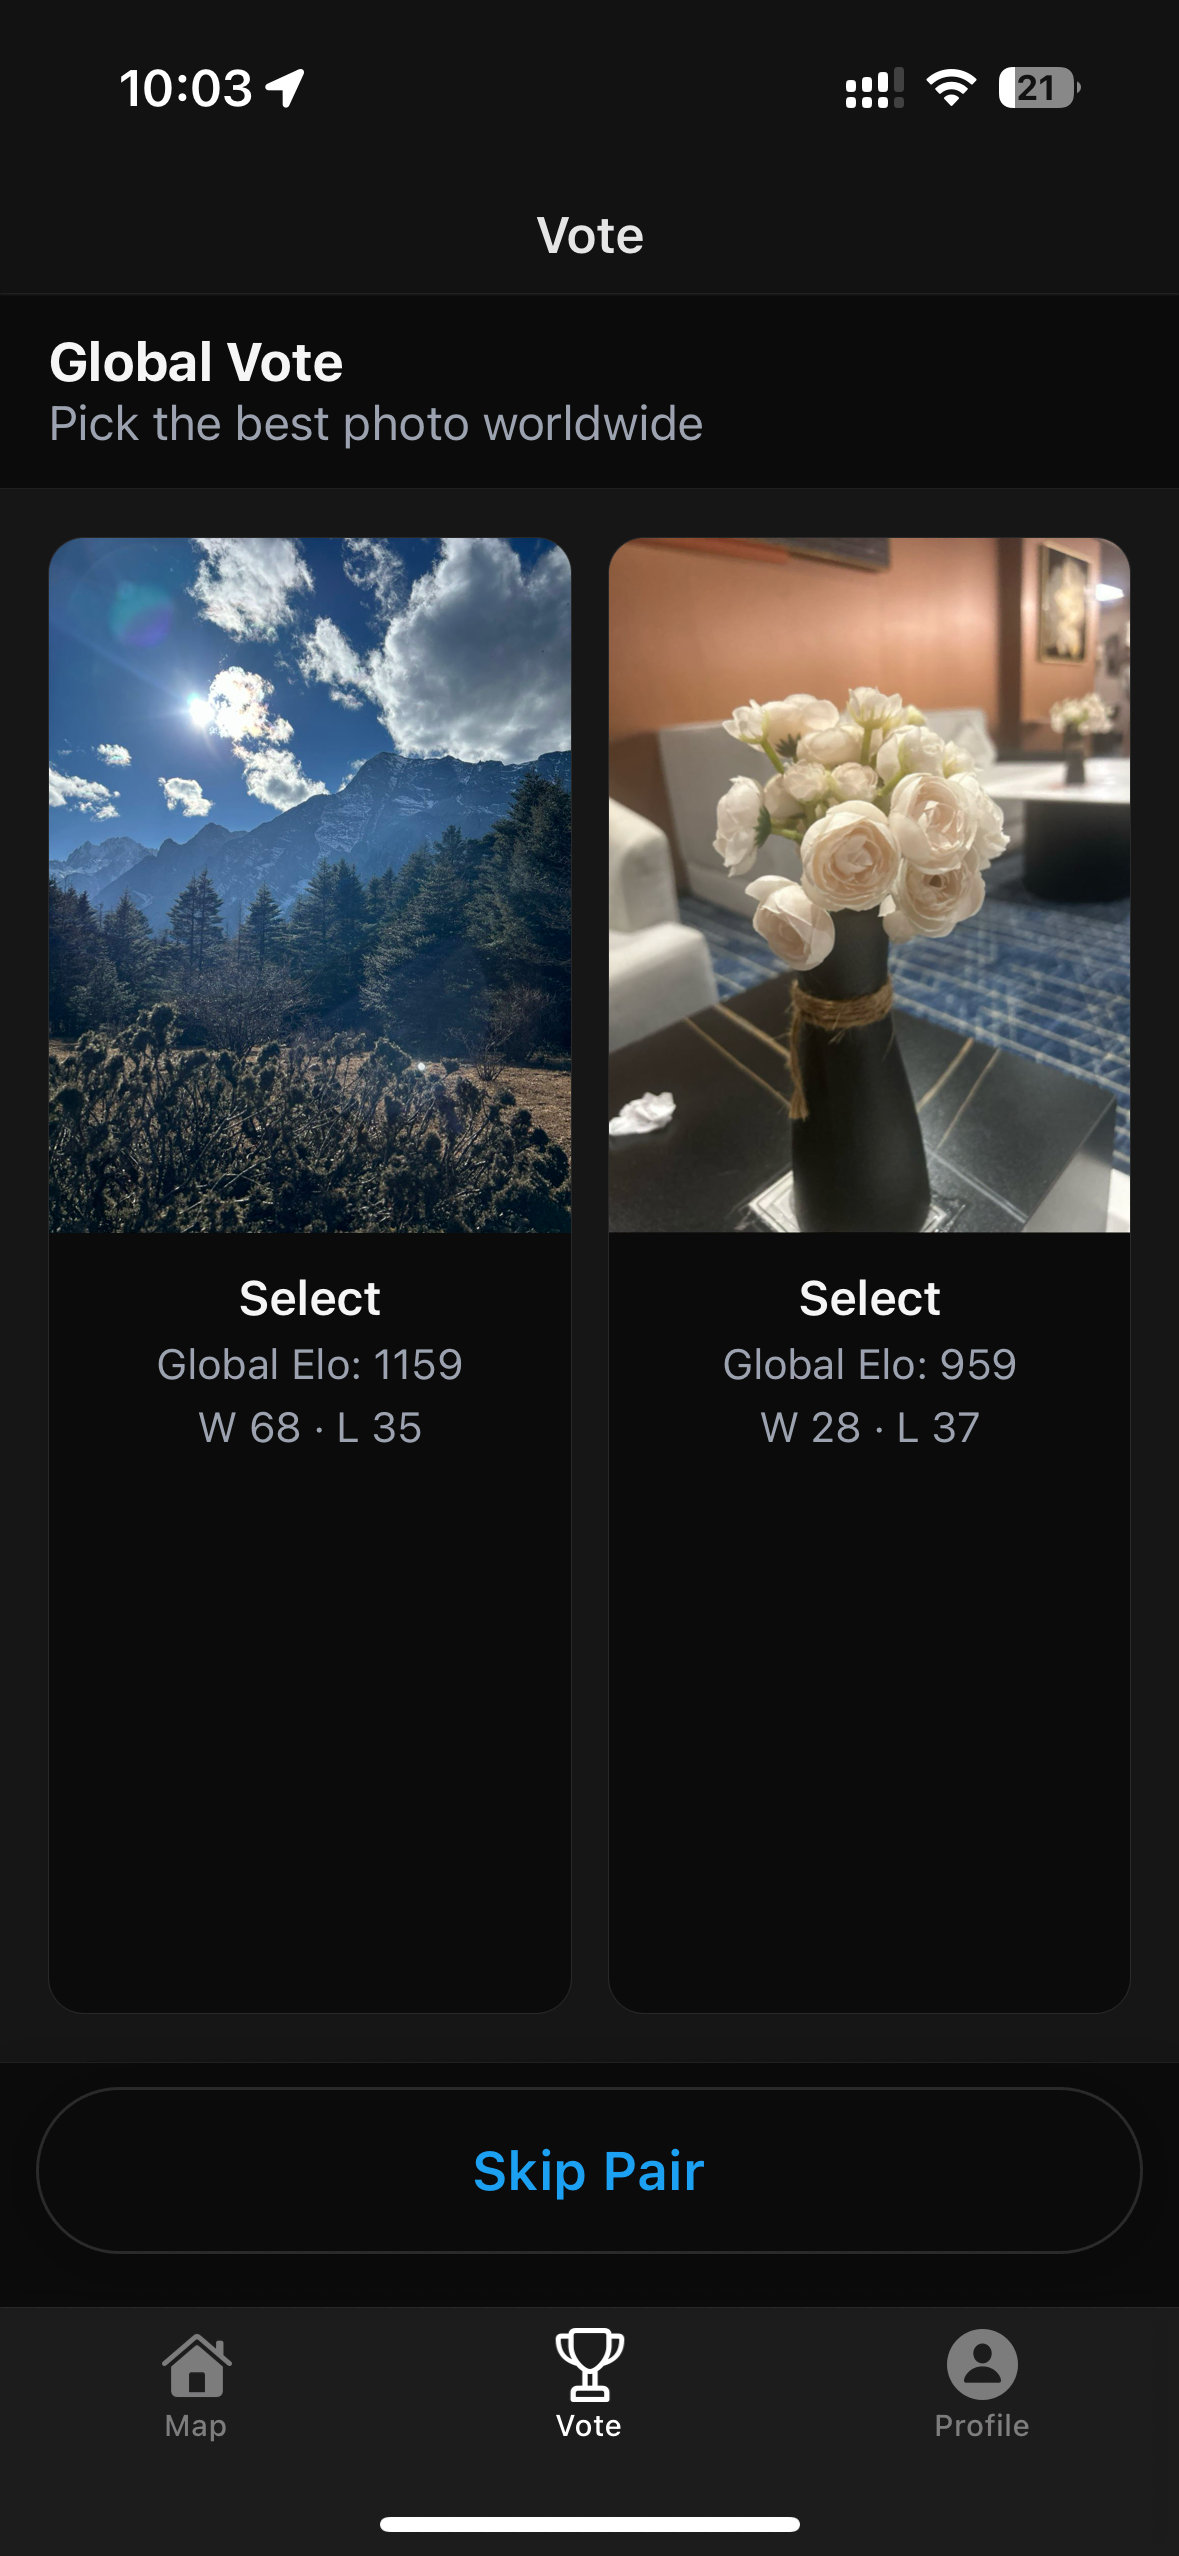
\includegraphics[width=\linewidth]{pre_vote.PNG}
\end{subfigure}
\hspace{2mm}
\begin{subfigure}{0.3\textwidth}
\centering
\includegraphics[width=\linewidth]{mid_vote.PNG}
\end{subfigure}
\hspace{2mm}
\begin{subfigure}{0.3\textwidth}
\centering
\includegraphics[width=\linewidth]{post_vote.PNG}
\end{subfigure}

\caption{Screenshots showing the vote screen throughout development.}
\label{fig:vote_before_after}
\end{figure}

However, needing to display two 3:4 photos on a vertical display proved a design challenge. The first redesign placed each photo in a card, with one in front of the other. Users could swipe left and right to select a card, then swipe up to declare it the winner. The feedback for this redesign was highly negative. Users said that even the basic tapping mechanic was better, as it didn't require multiple movements to select a photo.

The next redesign left the cards stacked on top of one another, but a swipe left or right would enlarge the card on that side to fill the whole screen. Releasing your finger at the end of the swipe would submit that photo as the winner, while leaving your finger on the display would let you keep looking at the photos. While this design allowed quick, one-movement voting, some users didn't even understand they were voting. Very few phone design elements require the finger to be pressed to the screen continuously to avoid submitting, and this movement was not intuitive to users as they just `swiped' to browse the photos just like in a photo gallery.

The final redesign put the photos directly on top of one another, with a `VS' divider that changed the view from one to the other. When the user dragged the divider past the submission threshold it would change color. On submission, a header would flash letting the user know they had just submitted a vote. Although the swiping/submission behavior was the same as before, the design evoked a more familiar `before/after' comparison and there were more explicit cues to let users know what was happening. This time, users understood and appreciated the voting feature.

\subsection{Feature Three: Private Quests}
Sometimes conversations with users led us to rethink aspects of SideQuest’s design philosophy. One such conversation ultimately resulted in the addition of private Quests.

\begin{figure}[!htbp]
\centering

\begin{subfigure}{0.3\textwidth}
\centering
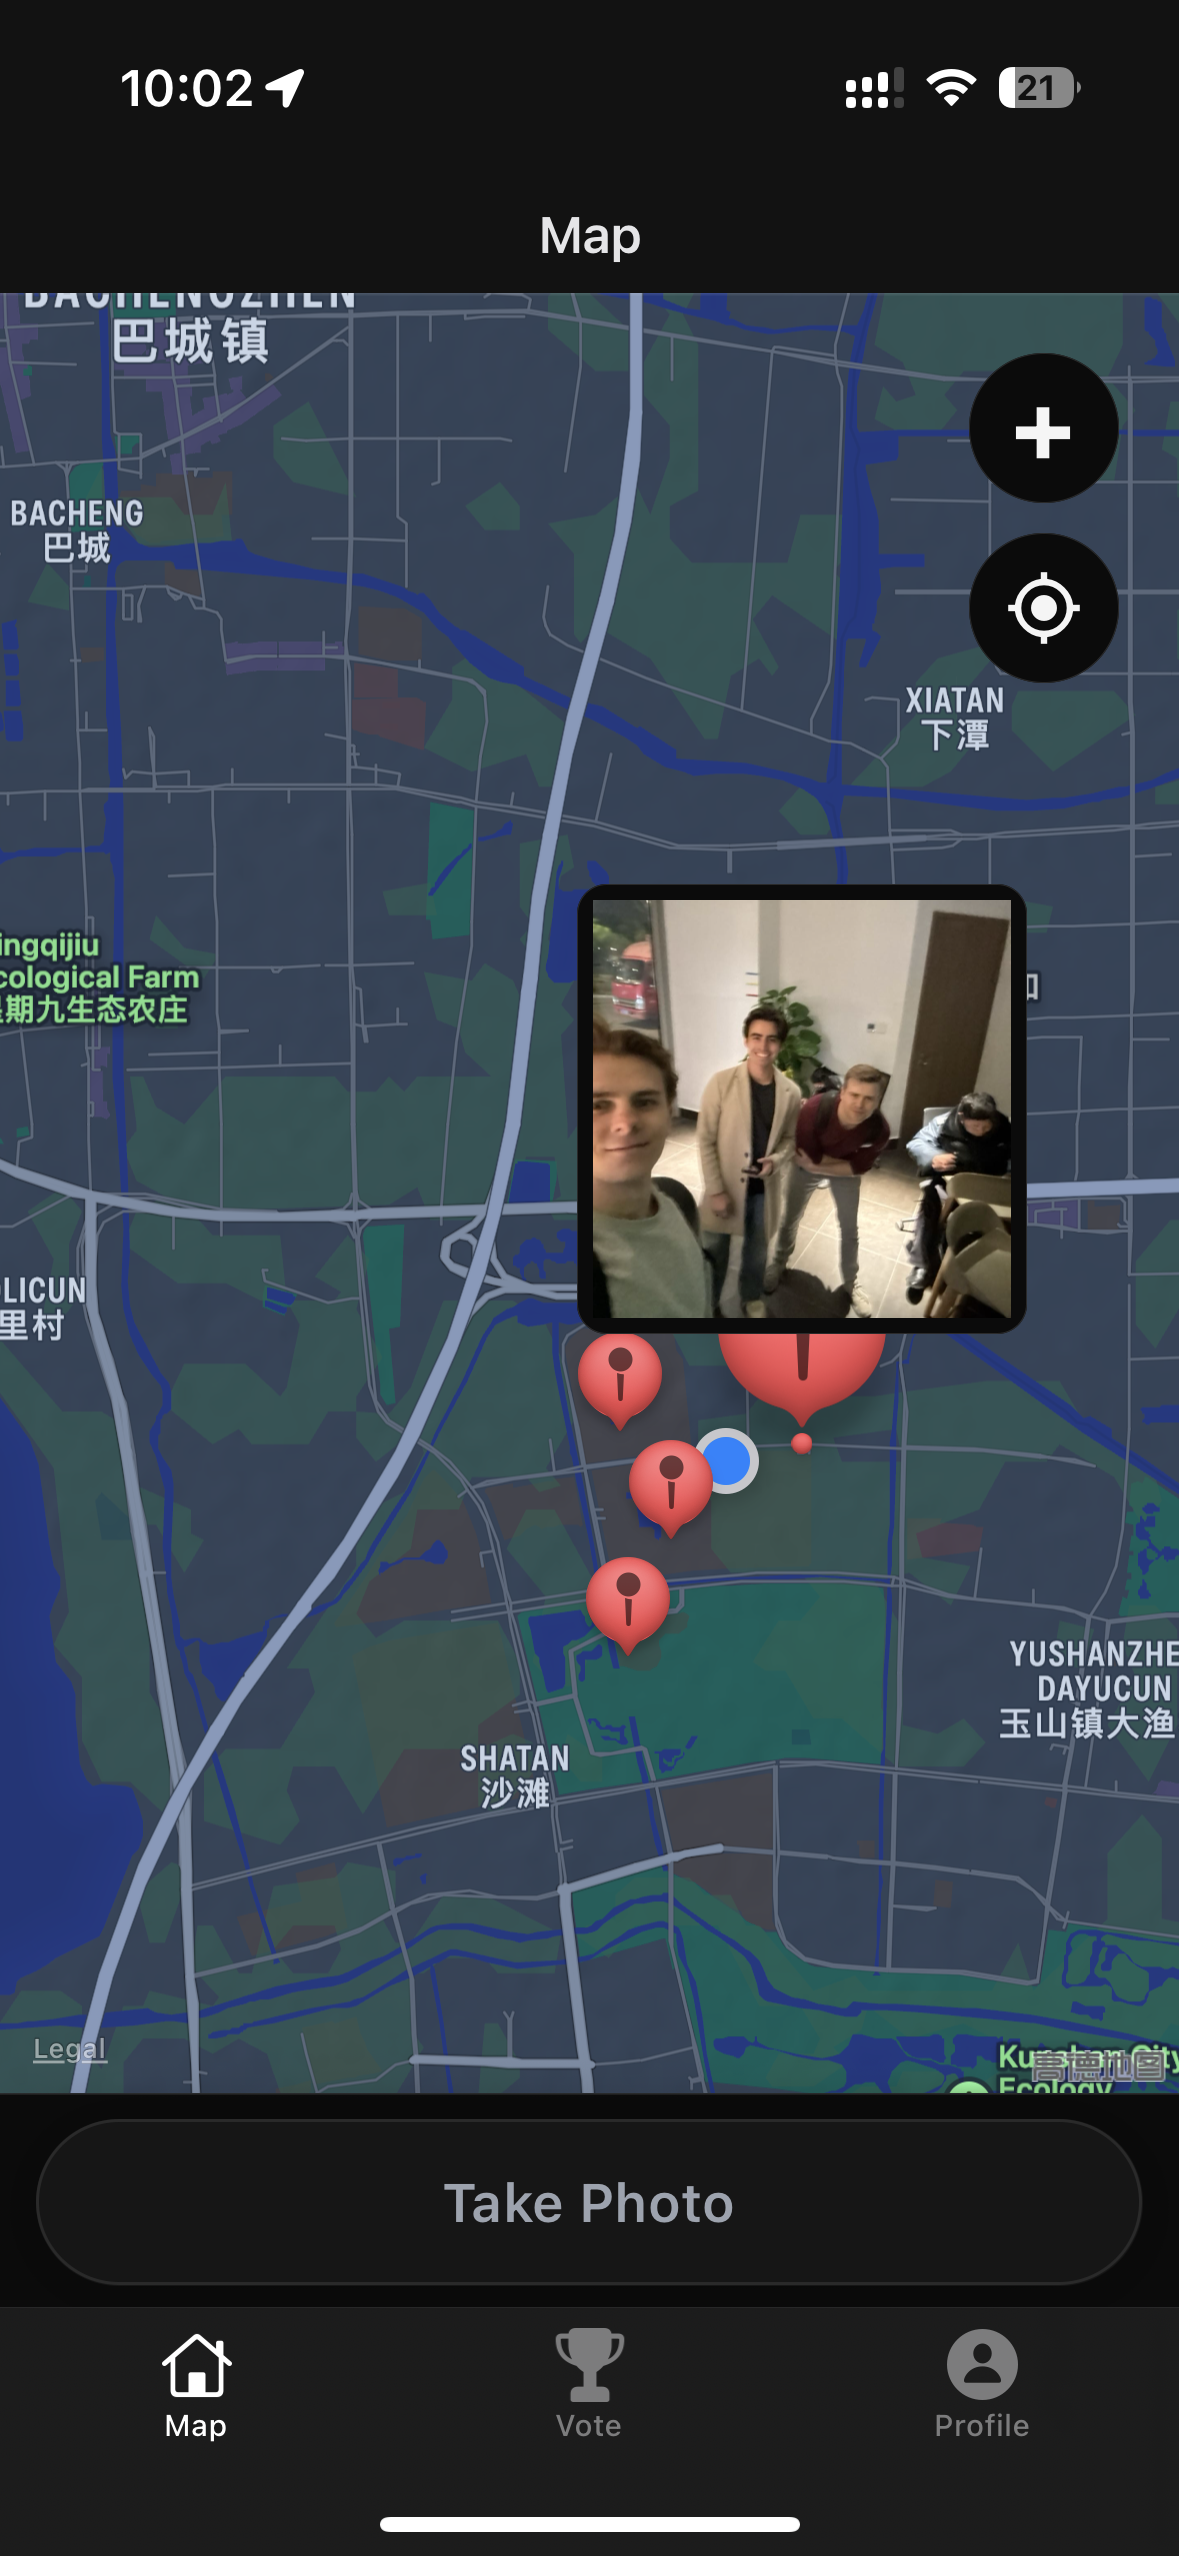
\includegraphics[width=\linewidth]{pre_private.PNG}
\caption{Quests on the map.}
\end{subfigure}
\hspace{2mm}
\begin{subfigure}{0.3\textwidth}
\centering
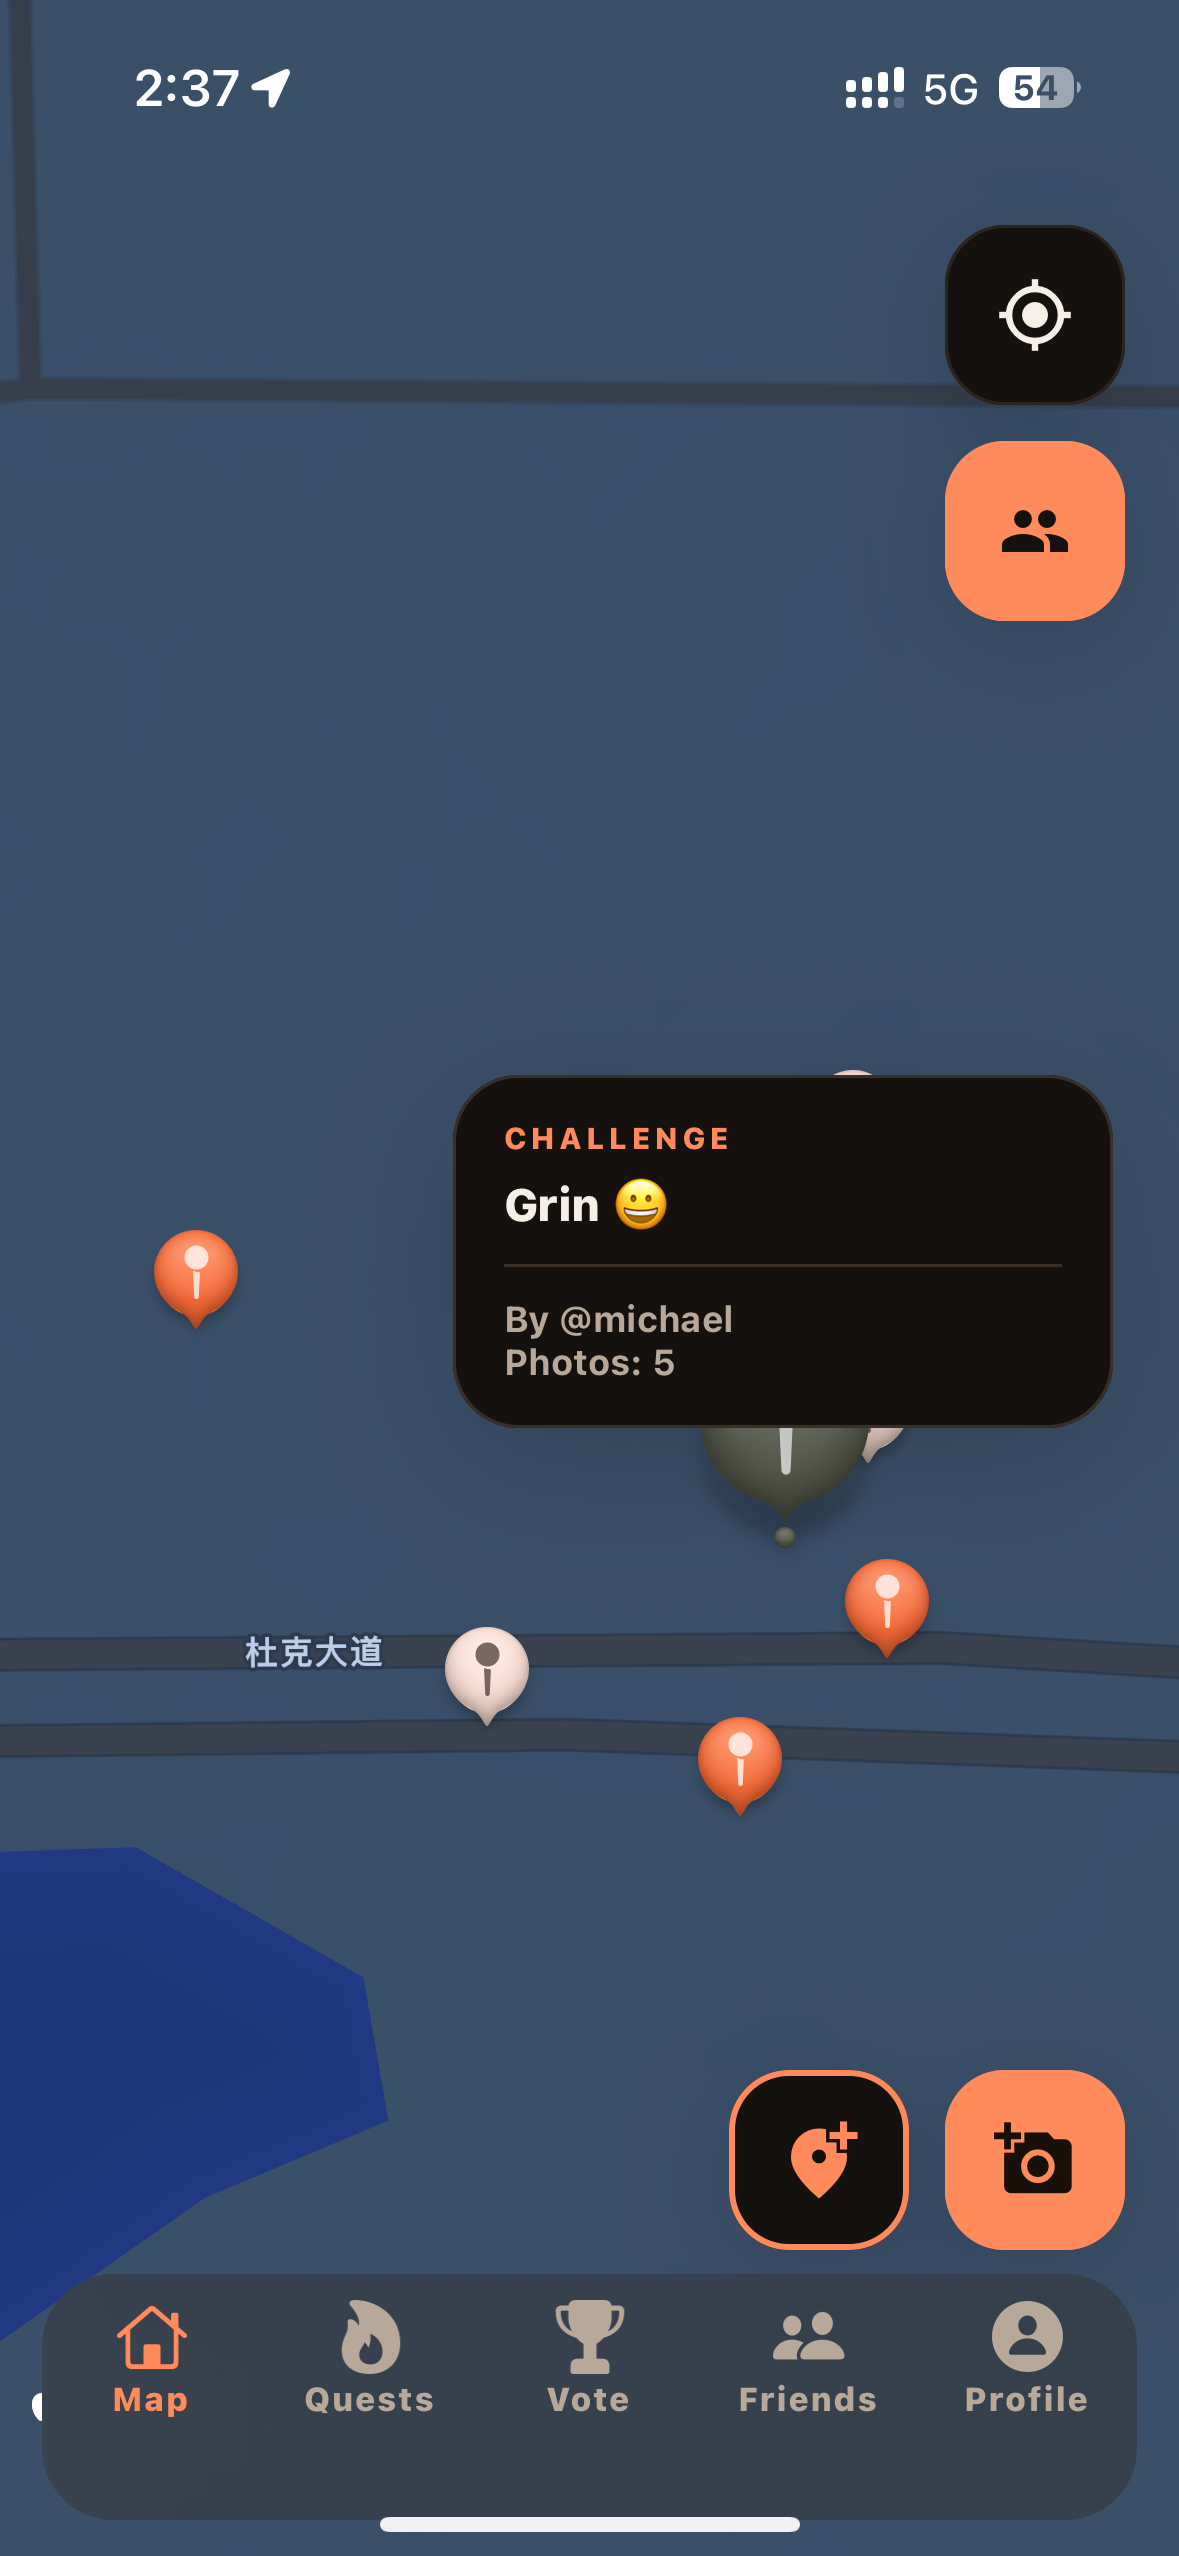
\includegraphics[width=\linewidth]{post_private1.PNG}
\caption{Private Quests are dark grey.}
\end{subfigure}
\hspace{2mm}
\begin{subfigure}{0.3\textwidth}
\centering
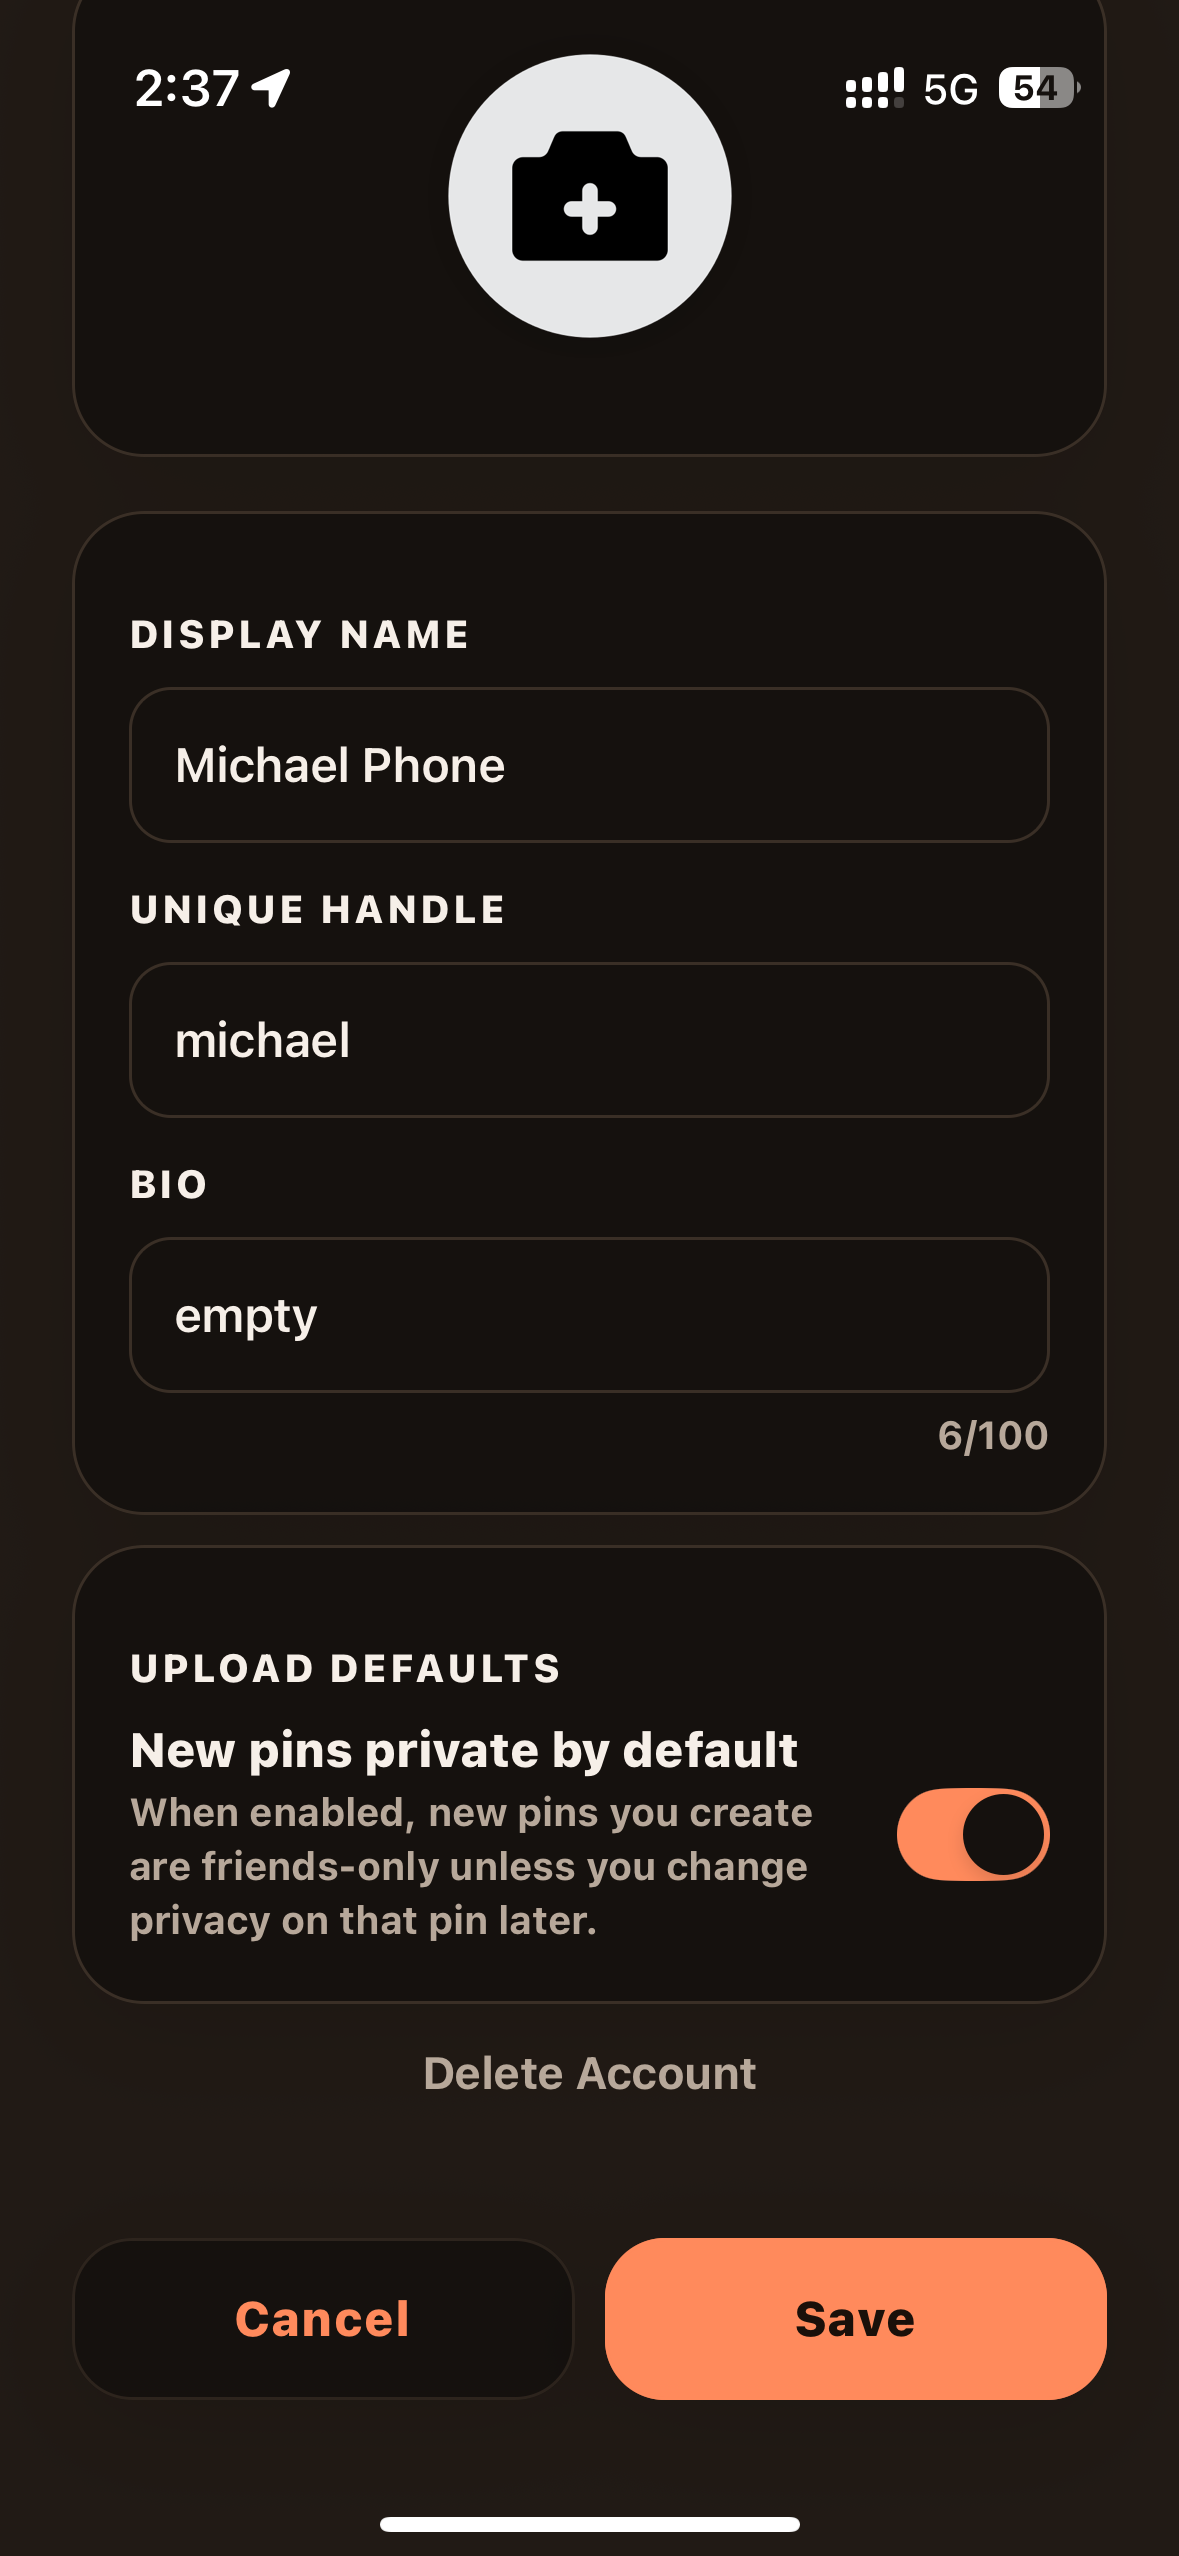
\includegraphics[width=\linewidth]{post_private2.PNG}
\caption{Setting to make Quests private by default.}
\end{subfigure}

\caption{Screenshots showing the development of private Quests.}
\label{fig:private_before_after}
\end{figure}

The user who raised this issue was almost the ideal type of SideQuest participant. He traveled extensively, enjoyed exploring new places, and wanted a way to document those experiences while sharing them with close friends. At first glance, SideQuest seemed like a perfect fit. However, during our conversation he mentioned that he did not use the app as often as he expected. The reason was simple: he only wanted his posts to be visible to his friends, not to the entire SideQuest community. Unlike many users, he did not use other social media platforms, and when he shared something online it was “only for his friends.”

Initially, Colden and I felt that this preference conflicted with the core idea of the app. The original concept assumed that if someone discovered a great location, they would create a Quest to encourage others to visit it as well. From the user’s perspective, however, the places he discovered felt personal, and he wanted the ability to decide whether or not to share them publicly. He did not want strangers appearing in locations that, to him, were part of a smaller circle of shared experiences.

After discussing this further, we realized that this perspective was reasonable and consistent with the broader goal of giving users meaningful control over their experiences. As a result, we introduced a privacy toggle in the Quest creation settings that allows a challenge to be marked as private, making it visible only to friends. We also added an option in the user settings to make all new Quests private by default.

% ============================================================================
\chapter{Final Outcome}
\label{ch:final}

\section{Concept Statement}
Born out of the gap between place based media and social media, SideQuest allows users to challenge others with a short photo prompt. Others can then see the challenge location and prompt on their map, but they have to travel to the place themselves to post their own attempt. The community then votes on the best photos, and winners earn badges. Over time, each location becomes an evolving, community-built collection of responses to a shared challenge.

SideQuest is implemented as a full-stack mobile application deployed on iOS and supported by a production backend. The system integrates location-based challenges, photo submission, and pairwise voting to create a structured but flexible environment for creative participation. Within the first three weeks of deployment, the application attracted 30 active daily users, who uploaded over a hundred photos, and cast over a thousand votes. While still early in its lifecycle, this initial activity demonstrates that the core interaction model—exploration, contribution, and comparison—functions under real usage conditions. 

\section{What is Delivered}
The complete list of delivered artifacts is provided in the Artifact Inventory in the Appendix (see Appendix~\ref{sec:artifact-inventory}).

\section{Example User Journey}

The next section follows Kailani, one of our test users, to demonstrate the app's features and interactions. The supporting screenshots for this walkthrough are collected in Appendix~\ref{sec:user-journey-figures}.

\textbf{Step 1: Notification and entry into voting.}
Kailani receives a push notification on her phone indicating that her votes have refreshed. Curious to see new content, she taps the notification directly from the lock screen (Fig.~\ref{fig:lock_notif}). The notification launches the SideQuest application and opens directly to the Vote tab.

\textbf{Step 2: Voting on photo duels.}
Inside the Vote tab, Kailani is presented with a pair of photos. She then swipes to her favorite, casting a vote that updates the rankings (Fig.~\ref{fig:vote}). The interface allows users to quickly compare contributions from across the platform.

\textbf{Step 3: Vote exhaustion reminder.}
After submitting all of her available votes, Kailani is shown a message indicating that voting has been exhausted for the current period (Fig.~\ref{fig:vote_exhaust}). This reminder encourages users to engage with other parts of the application rather than continuing to passively browse.

\textbf{Step 4: Browsing Quests.}
After finishing her votes, Kailani switches to the Quests tab to browse available prompts. She encounters a Quest titled “Play tag with your friends!” Although she cannot participate at the moment, she swipes upward to save the Quest for later  (Fig.~\ref{fig:save_quest}). 

\textbf{Step 5: Creating a new Quest.}
Kailani then navigates to the Map tab to create her own challenge. From her current location at a café, she takes a photo of the city view and writes the prompt “City view.” She chooses to allow anyone to participate in the challenge by disabling the “Location-Locked” option before pressing the CREATE button (Fig.~\ref{fig:create_city}).

\textbf{Step 6: Viewing the Quest on the map.}
After posting the challenge, Kailani is returned to the Map tab. Her newly created Quest now appears as a marker on the map (Fig.~\ref{fig:map_city}). The marker uses a color indicator showing that the Quest is open to participation from any user.

\textbf{Step 7: Viewing and editing the profile.}
Kailani next navigates to the Profile screen to see how creating the new Quest contributes to her progress toward platform badges (Fig.~\ref{fig:empty_profile}). Realizing she wants to personalize her account further, she taps the edit icon to open the profile editing interface (Fig.~\ref{fig:edit_profile}). Here she can update her display name, handle, biography, and default privacy settings for new Quests. After saving her changes, the app returns her to the profile screen.

\textbf{Step 8: Sharing the profile.}
To invite a friend to join the platform, Kailani taps the Share Profile button. This opens the system share sheet, allowing her to send a personalized invitation link (Fig.~\ref{fig:share}). The link directs her friend to install SideQuest and connect with her account.

\textbf{Step 9: Accepting a friend request.}
Finally, Kailani opens the Friends tab to manage her social connections. She sees an incoming friend request from the person she just invited and accepts it (Fig.~\ref{fig:friend}). This enables them to view each other’s private Quests on the map.

\section*{Conclusion}
SideQuest is a full-stack application following a common development lifecycle from design and development, to deployment and testing. Promising active user numbers shortly after the app's release provide evidence that the app can succeed at scale. Going forward, features will continue to be built out iteratively using user feedback, with the goal of building out a userbase of users that delight in the app.

%%%%%%%%%%%%%%%%%%%%%%%%%%%%%%%%%%%%%%%%%%%%%%%%%%%%%%%%%%%%%%%%%%%%%%%%%%%%%%%%
\chapter*{References}
\label{references}
\addcontentsline{toc}{chapter}{References}

\printbibliography[heading=none]

%%%%%%%%%%%%%%%%%%%%%%%%%%%%%%%%%%%%%%%%%%%%%%%%%%%%%%%%%%%%%%%%%%%%%%%%%%%%%%%%
\appendix

\chapter{Appendices}
\label{ch:appendices}

\section{Artifact Inventory}
\label{sec:artifact-inventory}
\textbf{Primary artifact}
\begin{itemize}
  \item SideQuest iOS App: \href{https://apps.apple.com/us/app/sidequest-explore-challenge/id6753264647}{App Store link}
\end{itemize}

\textbf{Secondary Artifacts}
\begin{itemize}
  \item Frontend and Backend GitHub Repositories (source code, commit history): \\
  \href{https://github.com/ColdenJohnson/geoapp}{Frontend repository}, \\ Backend repository (private GitHub repository)
  \item Deployed Backend (Docker container on Google Cloud Run): \\
  \href{https://geode-backend-834952308922.us-central1.run.app/}{Backend service endpoint (only accessible through SideQuest)}
  \item LaTex source for this paper \href{https://github.com/MicCorn/SignatureWorkPaper_SideQuest}{Source repository}
  \item Screenshots of App State
  \item Diagrams of database, tech stack, development workflow, etc.
\end{itemize}

\section{Ranking and Selection Equations}
\label{sec:ranking}
The Elo expected score for photo $A$ against photo $B$ is

\[
E_A = \frac{1}{1 + 10^{(R_B - R_A)/400}}
\]

and the corresponding rating update is

\[
R'_A = R_A + K(S_A - E_A)
\]

where $K = 24$, and $S_A = 1$ for the winning photo and $S_A = 0$ for the losing photo.

Weighted random selection is used in several places, including duel-lane choice and recency-biased pin selection. In general,

\[
P(i) = \frac{w_i}{\sum_j w_j}
\]

where $w_i$ is the weight assigned to option $i$.

For recency-biased pin selection, the implementation uses an exponential decay rule of the form

\[
w = 0.1 + 0.2 \cdot \exp\!\left(\frac{-\ln(2)\cdot \mathrm{ageHours}}{\mathrm{halfLife}}\right)
\]

with a half-life of 14 days. This gives newer pins more influence while preserving a nonzero floor for older pins.

\section{User Journey Figures}
\label{sec:user-journey-figures}

\begin{figure}[p]
\centering

\begin{subfigure}{0.32\textwidth}
\centering
\includegraphics[width=\linewidth]{lock_notif.PNG}
\caption{Push notification on the device lock screen prompting the user to return and vote.}
\label{fig:lock_notif}
\end{subfigure}
\hfill
\begin{subfigure}{0.32\textwidth}
\centering
\includegraphics[width=\linewidth]{vote.PNG}
\caption{Head-to-head voting interface. Users swipe to select their preferred submission.}
\label{fig:vote}
\end{subfigure}
\hfill
\begin{subfigure}{0.32\textwidth}
\centering

\includegraphics[width=\linewidth]{vote_exhaust.PNG}
\caption{Voting exhaustion message reminding users to use other parts of the app.}
\label{fig:vote_exhaust}
\end{subfigure}

\caption{Screenshots for Steps 1--3 of the example user journey.}
\label{fig:voting_pair}
\end{figure}

\begin{figure}[p]
\centering

\begin{subfigure}{0.32\textwidth}
\centering
\includegraphics[width=\linewidth]{save_quest.PNG}
\caption{Saving a Quest for later participation.}
\label{fig:save_quest}
\end{subfigure}
\hfill
\begin{subfigure}{0.32\textwidth}
\centering
\includegraphics[width=\linewidth]{create_city.PNG}
\caption{Creating a new Quest with a prompt and photo.}
\label{fig:create_city}
\end{subfigure}
\hfill
\begin{subfigure}{0.32\textwidth}
\centering
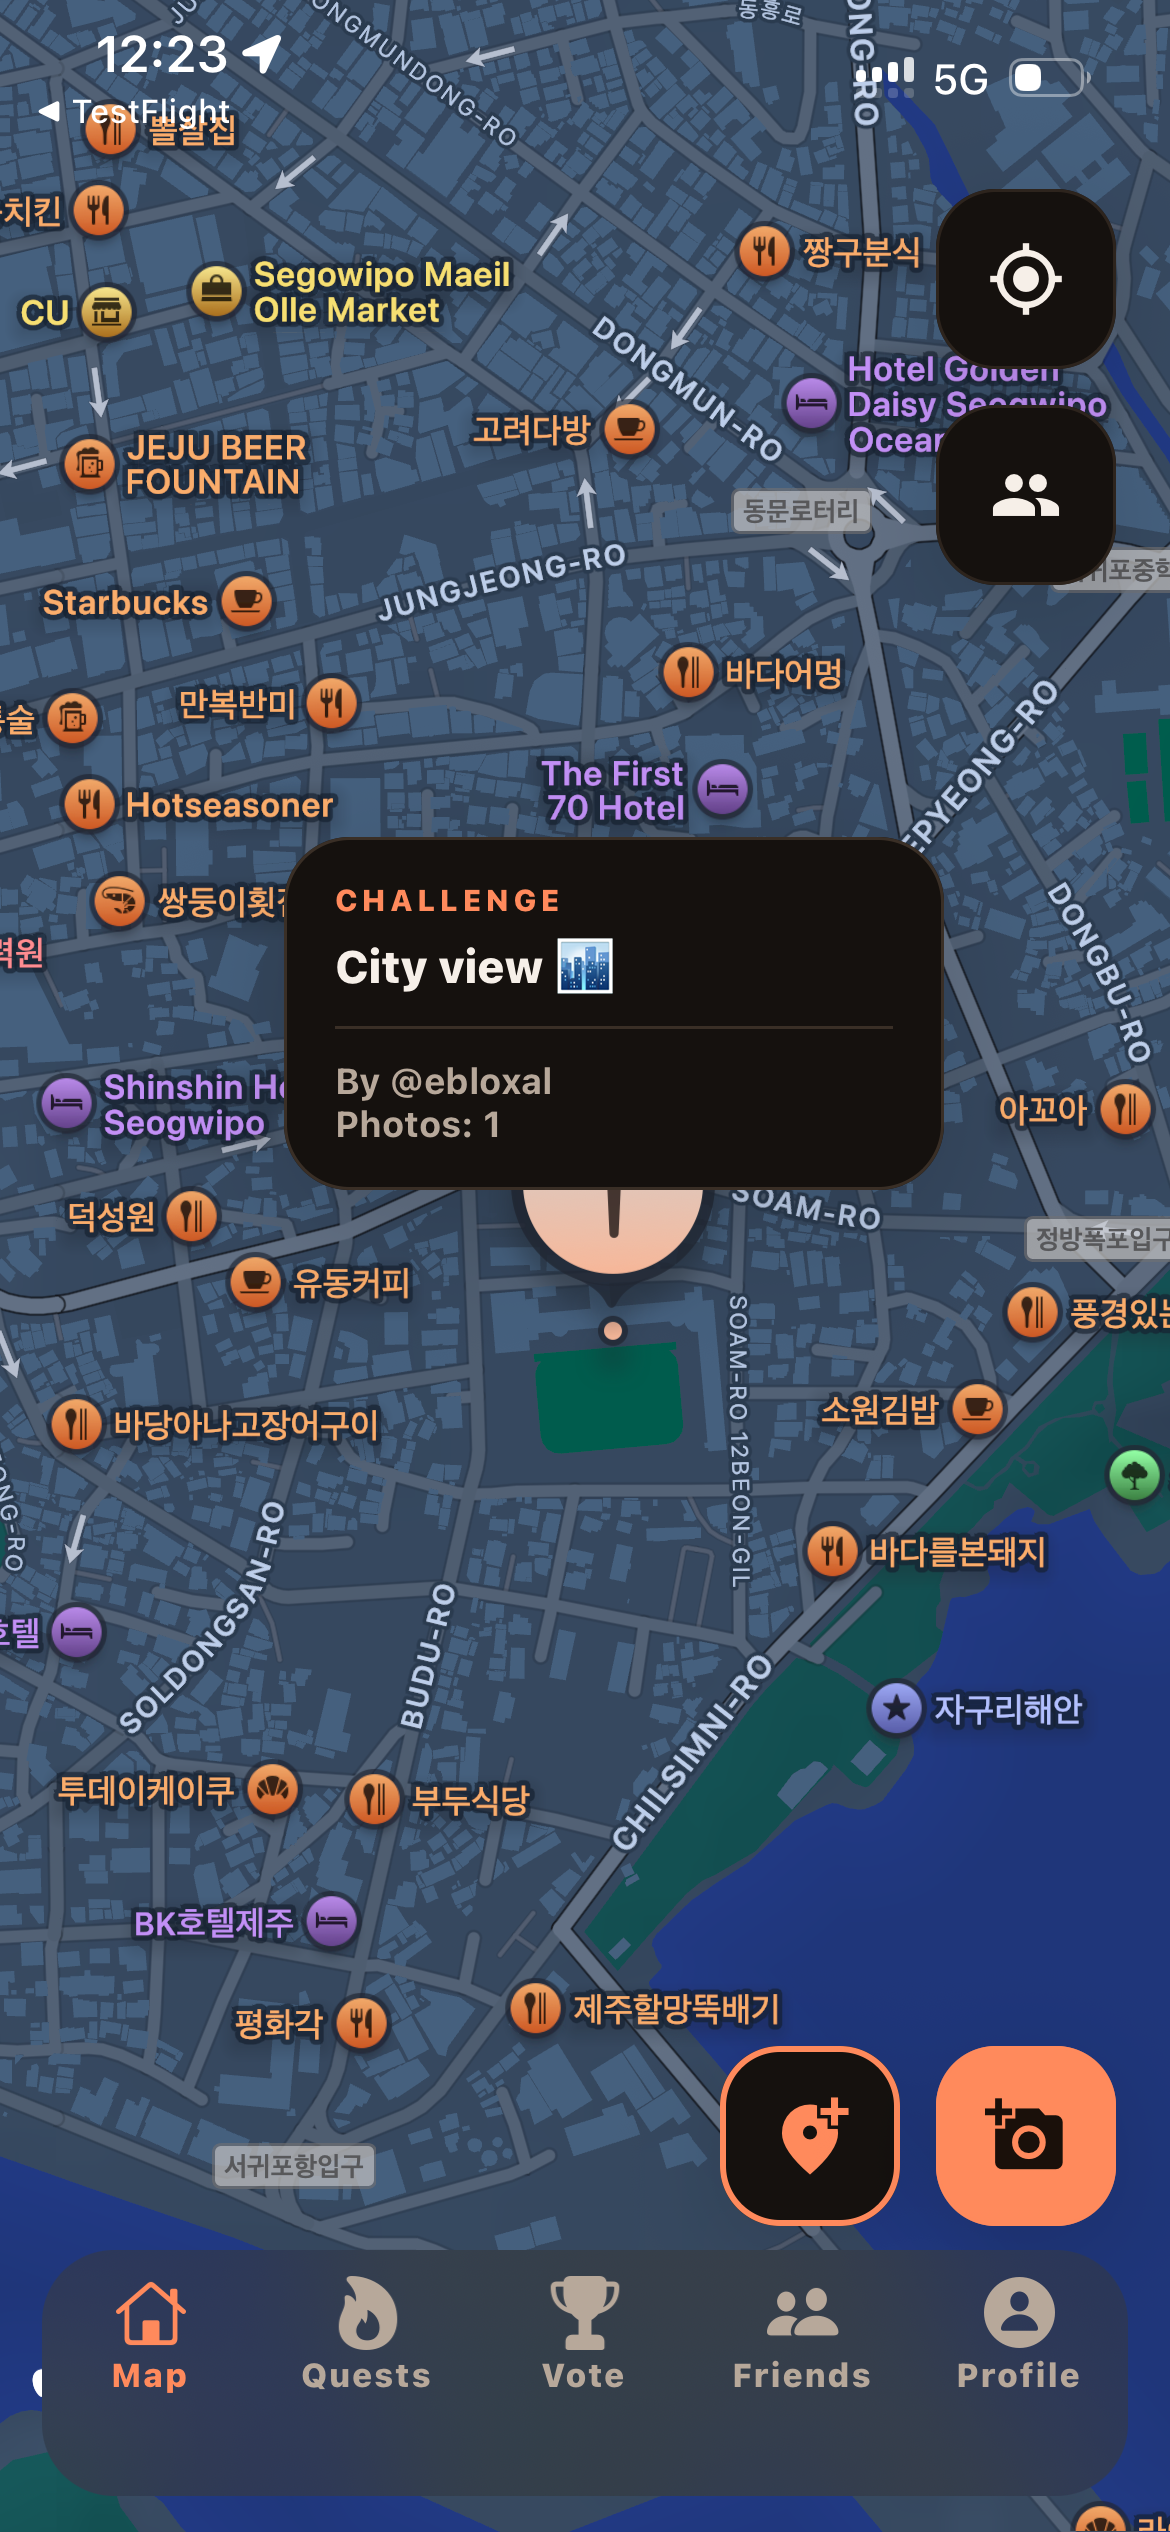
\includegraphics[width=\linewidth]{map_city.PNG}
\caption{A newly created Quest appearing on the map interface.}
\label{fig:map_city}
\end{subfigure}

\caption{Screenshots for Steps 4--6 of the example user journey.}
\end{figure}

\begin{figure}[p]
\centering

\begin{subfigure}{0.4\textwidth}
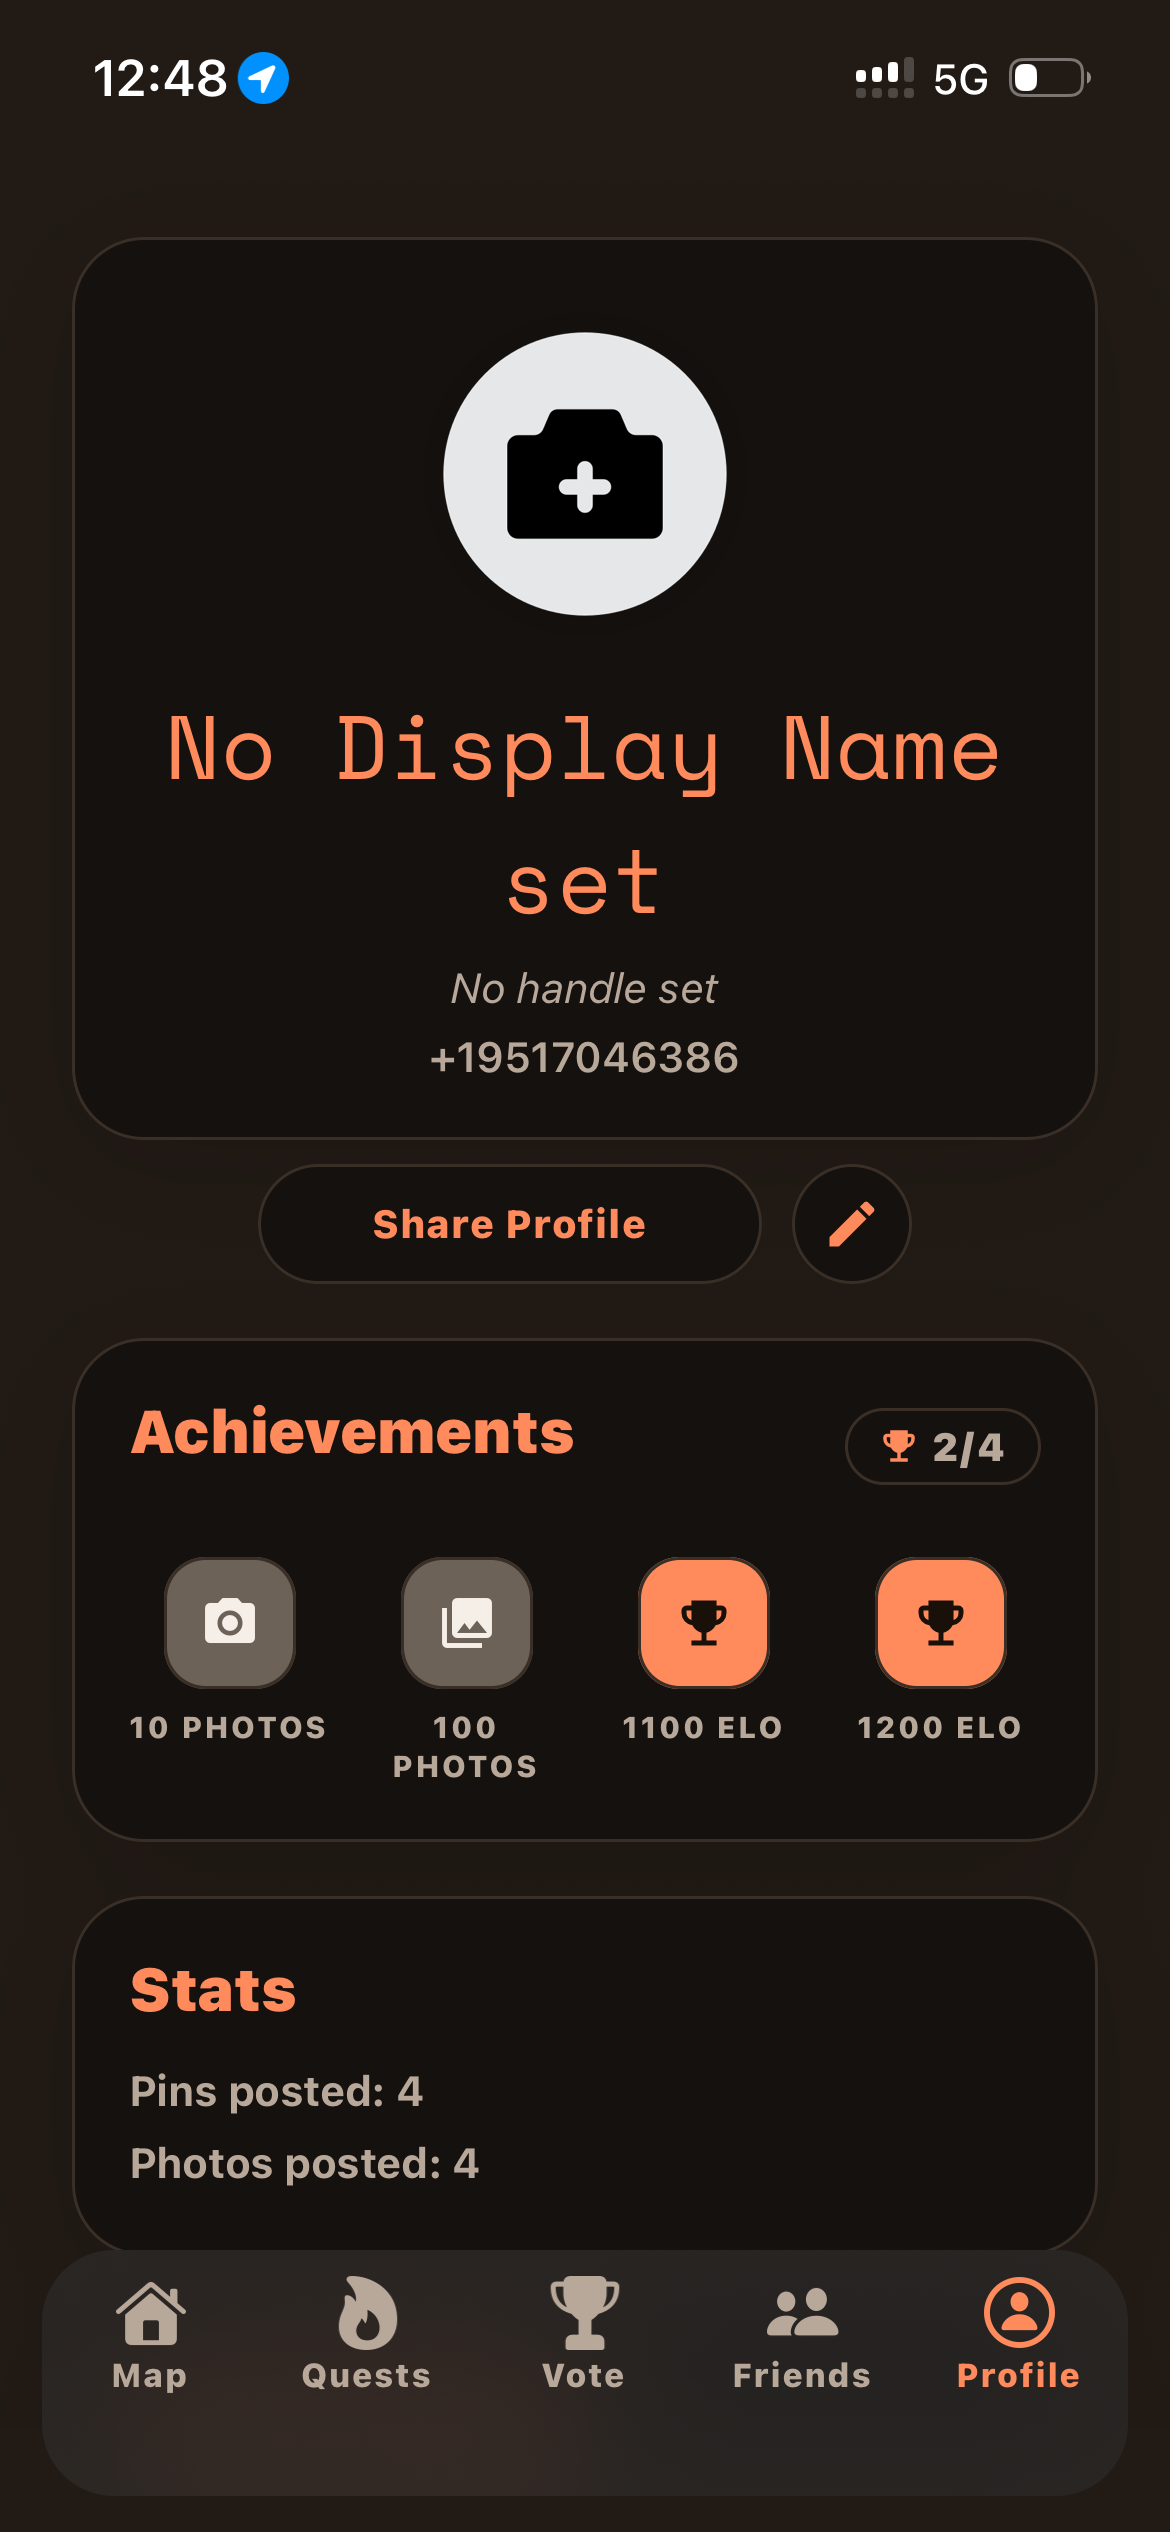
\includegraphics[width=\linewidth]{empty_profile.PNG}
\caption{User profile screen displaying progress and personal information.}
\label{fig:empty_profile}
\end{subfigure}
\hspace{4mm}
\begin{subfigure}{0.4\textwidth}
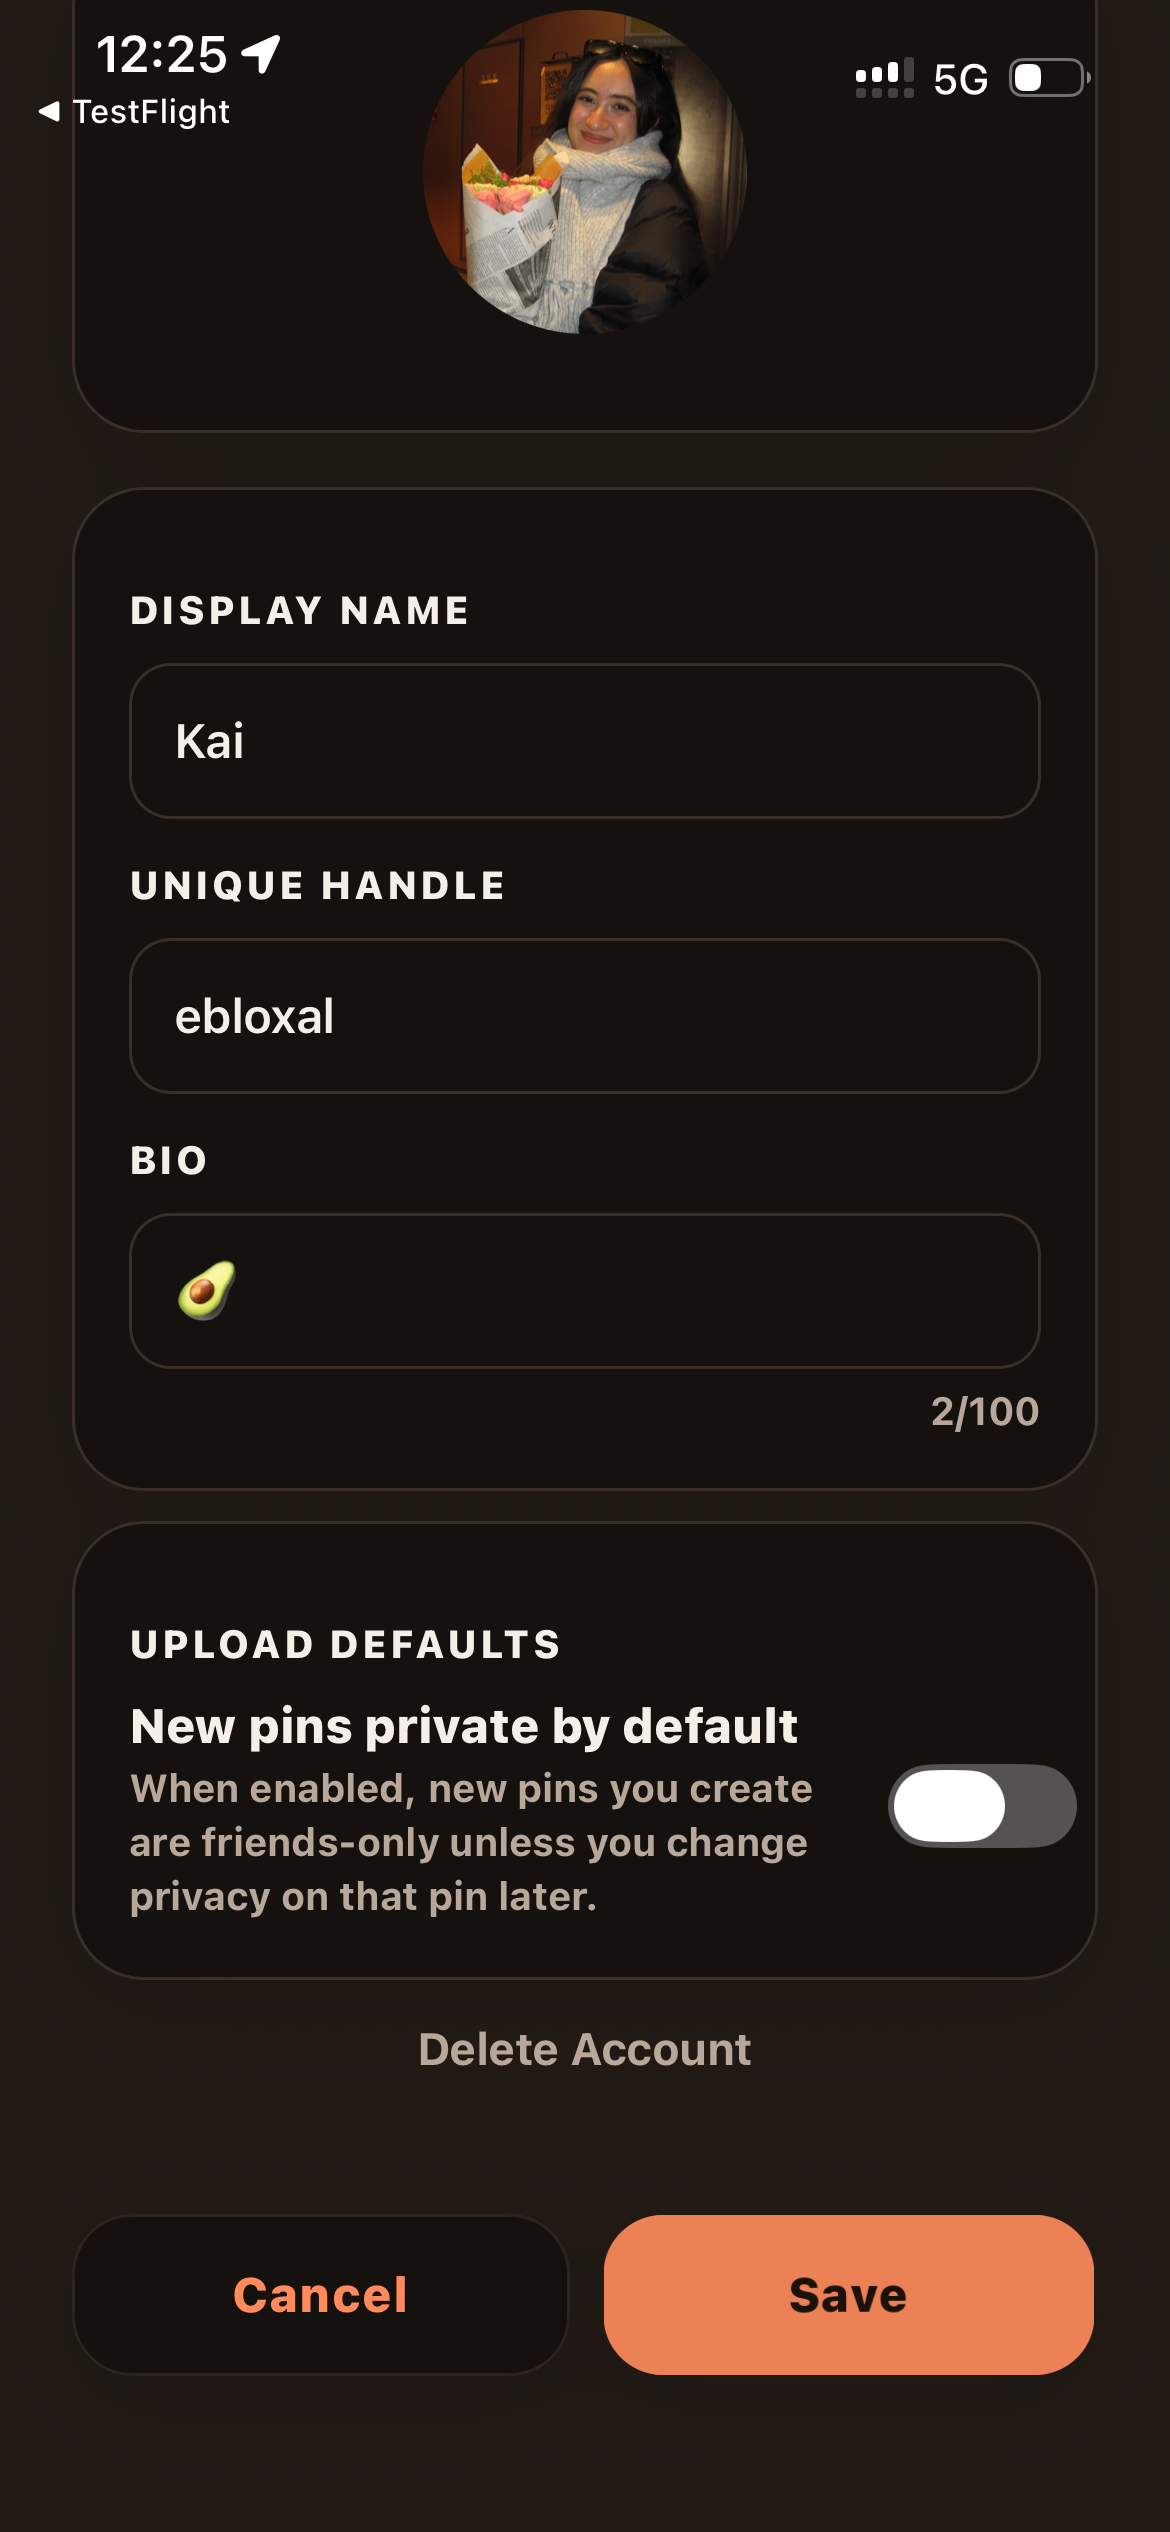
\includegraphics[width=\linewidth]{edit_profile.PNG}
\caption{Profile editing interface allowing users to update personal information and privacy settings.}
\label{fig:edit_profile}
\end{subfigure}

\caption{Screenshots for Step 7 of the example user journey.}
\end{figure}

\begin{figure}[p]
\centering

\begin{subfigure}{0.4\textwidth}
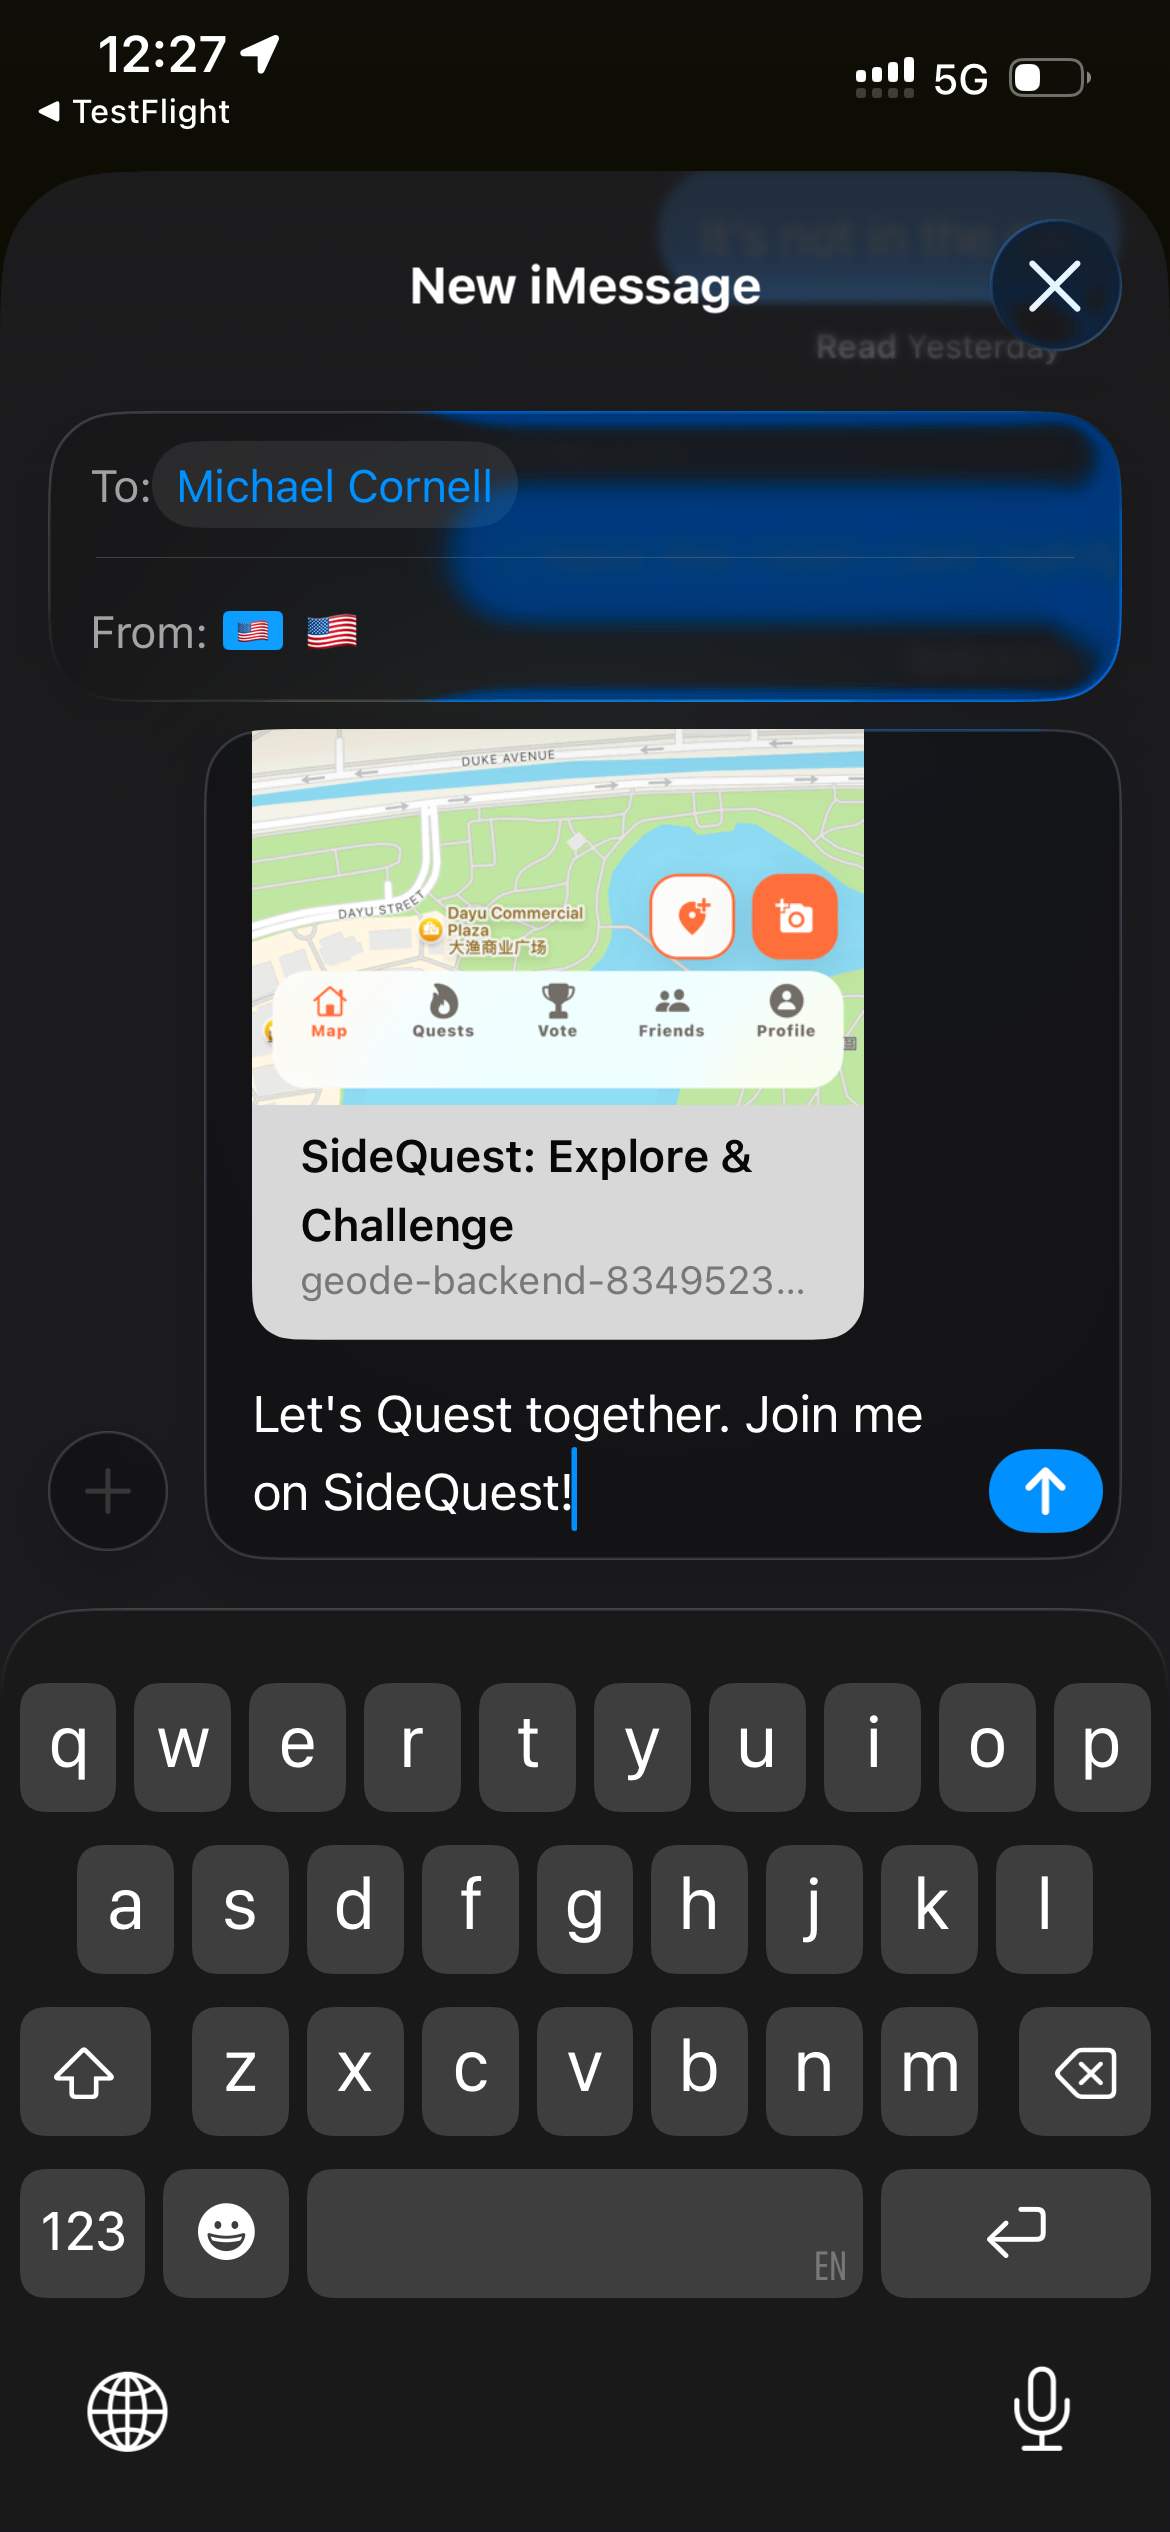
\includegraphics[width=\linewidth]{share.PNG}
\caption{Sharing a profile link through the system messaging interface.}
\label{fig:share}
\end{subfigure}
\hspace{4mm}
\begin{subfigure}{0.4\textwidth}
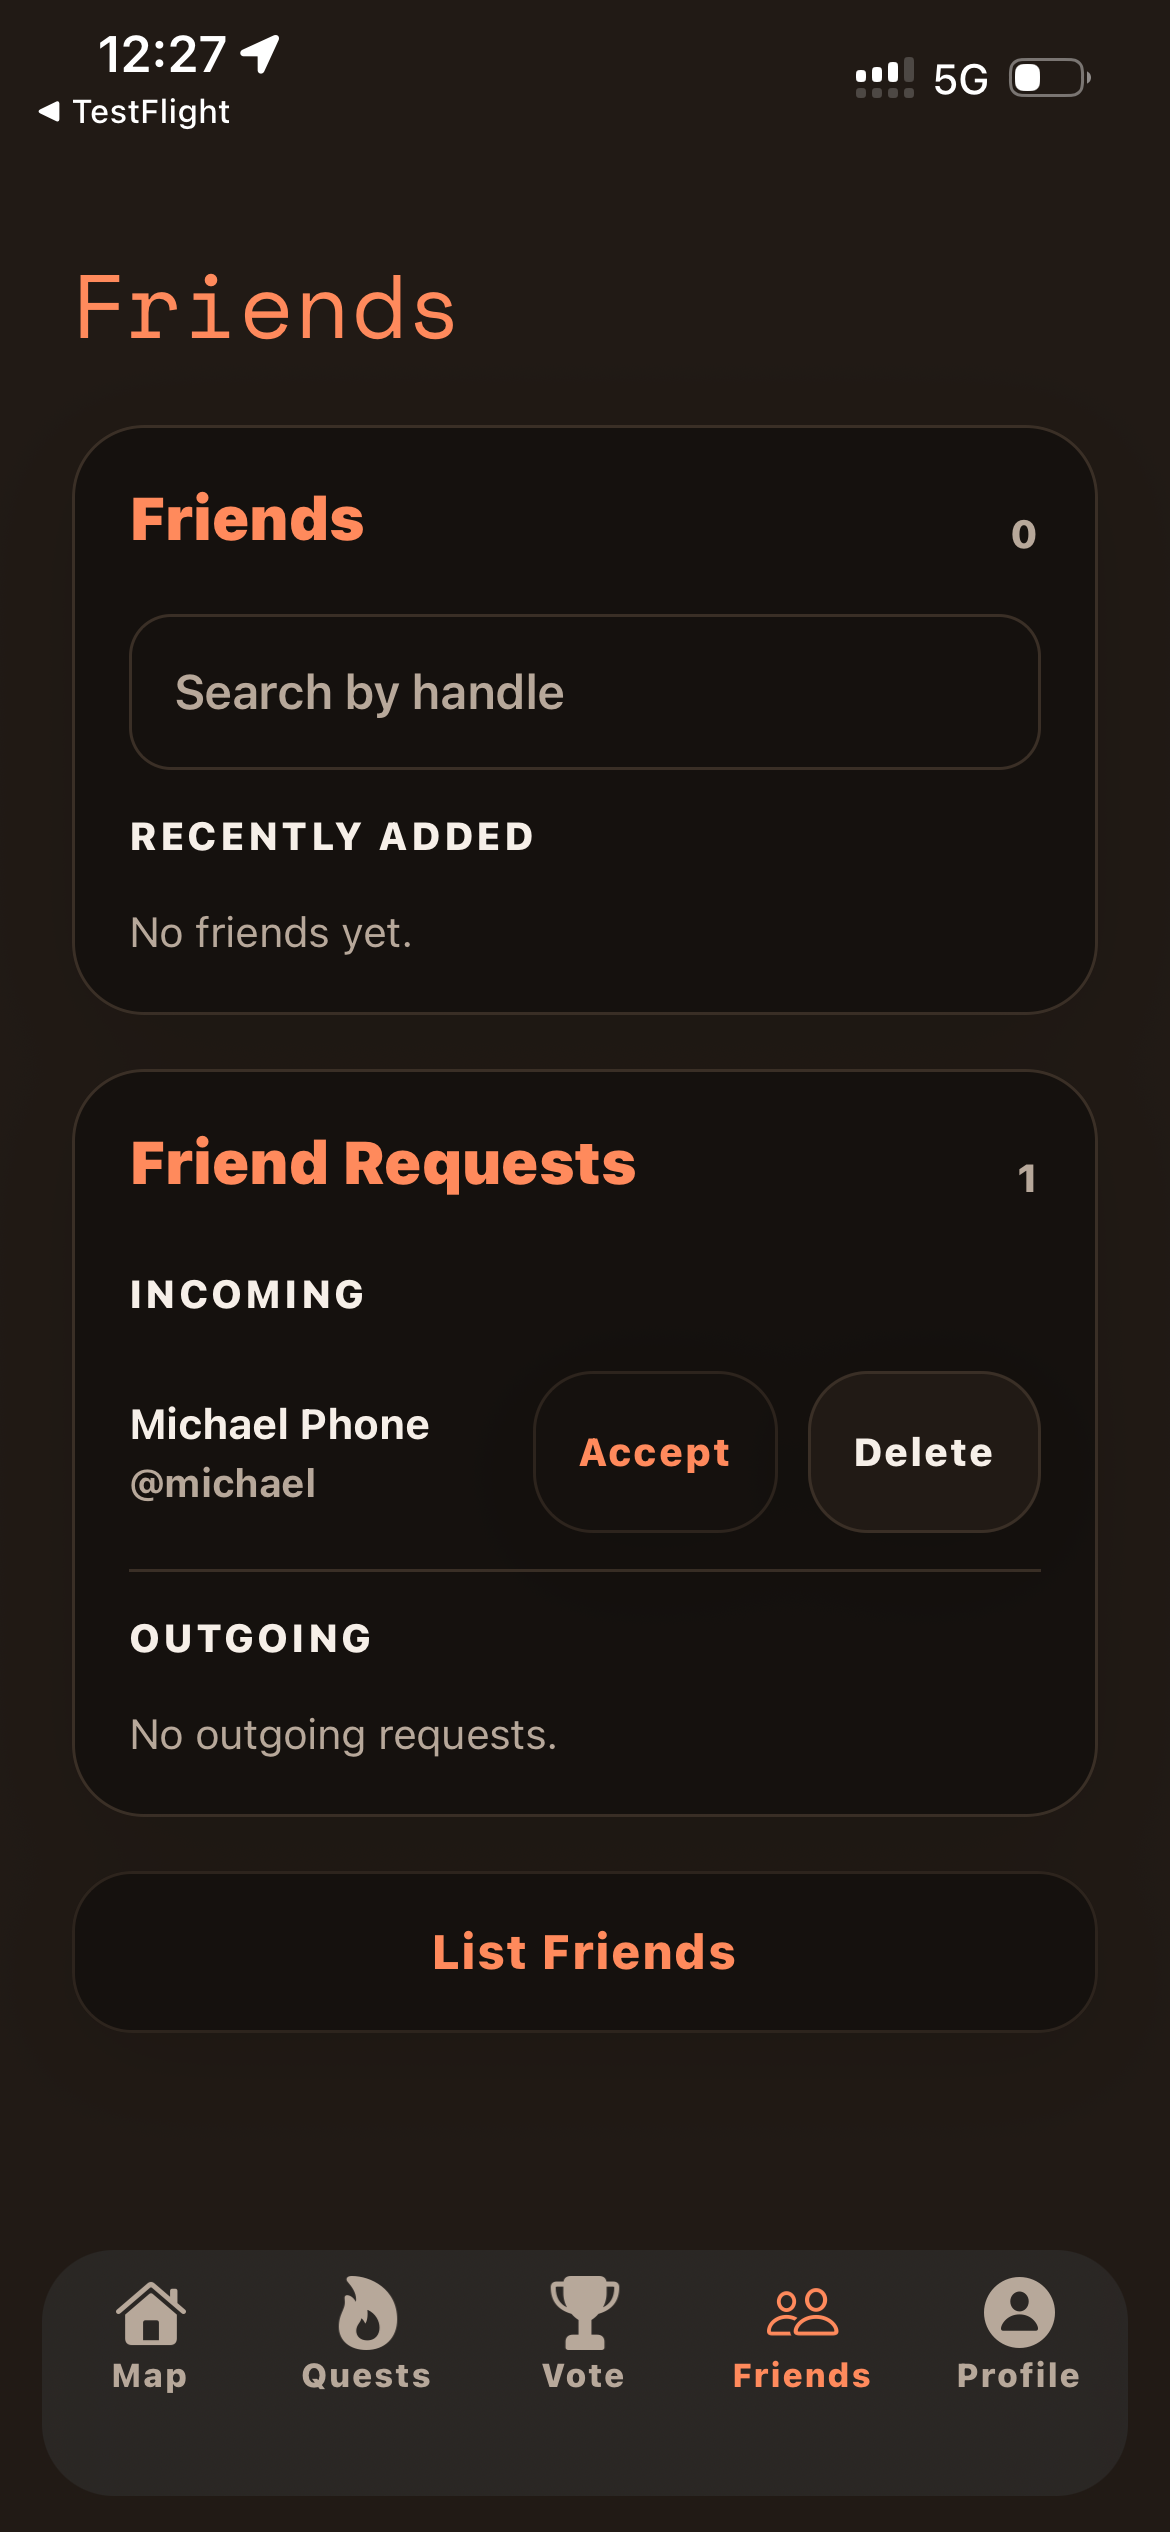
\includegraphics[width=\linewidth]{friend.PNG}
\caption{Accepting an incoming friend request in the Friends interface.}
\label{fig:friend}
\end{subfigure}

\caption{Screenshots for Steps 8--9 of the example user journey.}
\end{figure}

\end{document}
